\chapter[Results]{Results}

This chapter presents calculation results based on the methodology described in Chapters 3 and 4. The effective multiplication factor, number density of major isotopes, and $^{232}$Th refill rate are calculated using a full-core SERPENT 2 model with 3-day depletion steps over a 20-year time frame. Moreover, neutron flux, neutron energy spectrum, temperature reactivity coefficients, control rod worth, power density, and $^{233}$U breeding density distribution are presented for both initial and equilibrium fuel salt composition. The neutron flux and energy spectrum are calculated for the full-core model, normalized by neutron lethargy and reported for each zone. The temperature coefficients of reactivity for both the fuel salt and graphite components are estimated at the initial state by comparing effective multiplication factors at temperatures uniformly distributed from 900K and 1000K. The rod worth is calculated at several different insertion levels of control and safety rods. Finally, six factor analysis was performed to show evolution of these parameters during reactor operation.

The neutron population per cycle and the number of active/inactive cycles were chosen to obtain balance between reasonable uncertainty for a transport problem ($\leq$ 40 pcm for effective multiplication factor) and computational time. The \gls{MSBR} depletion and safety parameter computations were performed on 64 Blue Waters XK7 nodes (two AMD 6276 Interlagos CPU per node, 16 floating-point bulldozer core units per node or 32 ``integer" cores per node, nominal clock speed is 2.45 GHz). The total computational time for achieving equilibrium composition was approximately 9000 node hours (288,000 core hours.)

\section{Effective multiplication factor}
Figure~\ref{fig:keff} demonstrates the effective multiplication factors obtained using SaltProc and SERPENT 2. The effective multiplication factors are calculated after removing fission products listed in Table~\ref{tab:reprocessing_list} and adding the fertile material at the end of ``cycle time"\footnote{The \gls{MSBR} program defined a ``cycle time" as the amount of time required to remove 100\% of a target nuclide from a fuel salt.} which was fixed on 3 days for this work. The effective multiplication factor significantly fluctuates as a result of the batch-wise nature of this online reprocessing strategy. 
\begin{figure}[hbp!] % replace 't' with 'b' to 
  \centering
  \vspace{-0.3em}
  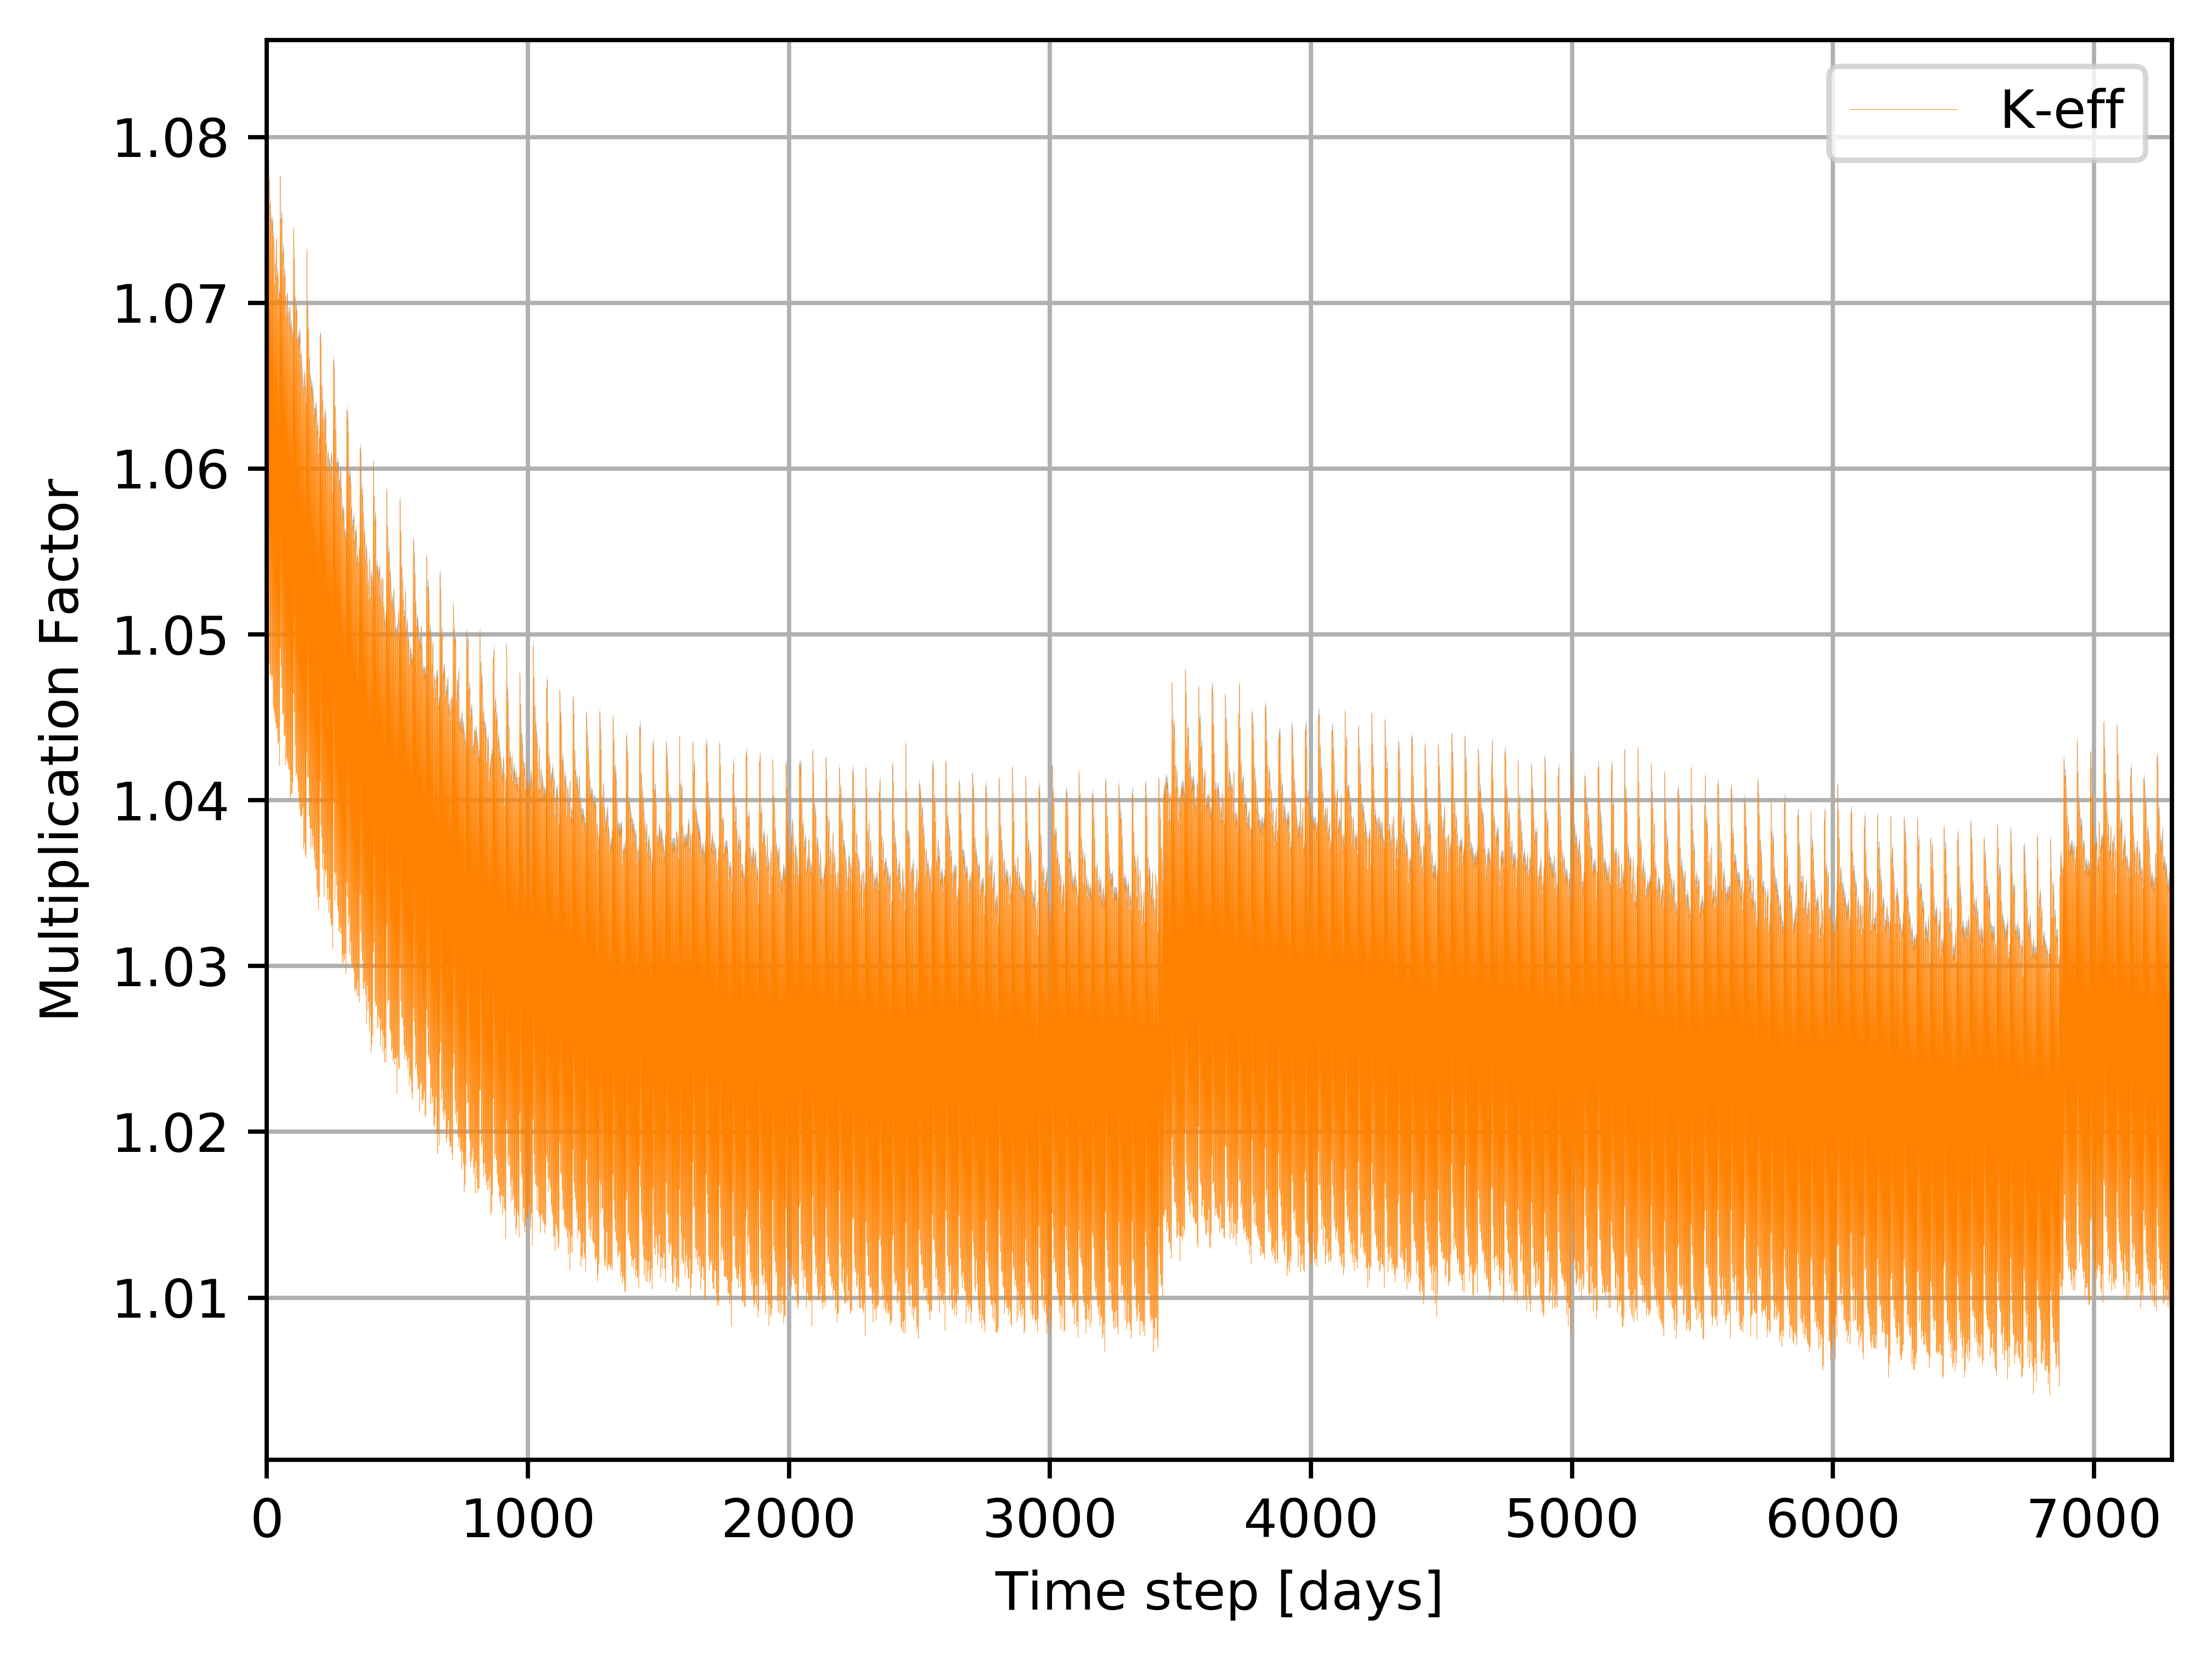
\includegraphics[width=1.05\textwidth]{keff.png}
  \caption{Effective multiplication factor dynamics for full-core \gls{MSBR} model for a 20-year reactor operation. The confidence interval $\pm\sigma$ is shaded.}
  \vspace{-0.6em}
  \label{fig:keff}
\end{figure}
\FloatBarrier

First, SERPENT calculates the effective multiplication factor for the beginning of cycle time (fresh fuel composition for the first step). Next it computes the new fuel salt composition for the end of a 3-day depletion step. The corresponding effective multiplication factor is much smaller than the previous one. Finally, SERPENT calculates $k_{eff}$ for the depleted composition after applying feeds and removals, and this increases accordinglysince major reactor poisons (e.g. Xe, Kr) are removed while fresh fissile material ($^{233}$U) from the protactinium decay tank is added. 

Additionaly, the presence of rubidium, strontium, cesium, and barium in the core are disadvantageous to reactor physics. In fact, removal of these elements every 3435 days causes the multiplication factor to jump by approximately 450 pcm, and limits using the batch approach for online reprocessing simulation. Overall, the effective multiplication factor gradually decreases from 1.075 to $k_{eff} \approx 1.02$ at equilibrium after approximately 6 years of irradiation. 

The analysis of the fuel salt composition evolution provides more comprehensive information about the equilibrium state. Figure~\ref{fig:adens_eq} shows major nuclides which have a strong influence on the reactor core physics normalized by average atomic density, at the beginning of each depletion time step.Concentration of $^{233}$U, $^{232}$Th, $^{233}$Pa, and $^{232}$Pa in fuel salt change insignificantly after approximately 2500 days of operation. Particularly, $^{233}$U number density fluctuates less than 0.8\% in the time interval from 16 to 20 years of operation, hence,a quasi-equlibrium state was achieved after 16 years of reactor operation.

In contrast, a wide variety of nuclides, including fissile isotopes (e.g. $^{235}$U) and non-fissile strong absorbers (e.g. $^{234}$U), keep accumulating in the core. Figures~\ref{fig:fissile_short}, \ref{fig:fissile_long} demonstrate production of short-life and long-life fissile isotopes in the core, respectively. In the end of considered operational time the core contains significant $^{235}$U ($\approx 9\times10^{-6}$ atom/b-cm), $^{238}$Pu ($\approx 10^{-6}$ atom/b-cm), $^{237}$Np ($\approx10^{-6}$ atom/b-cm), $^{232}$U ($\approx$10$^{-7}$ atom/b-cm), $^{239}$Pu ($\approx10^{-7}$ atom/b-cm), and $^{241}$Pu ($\approx 5\times10^{-8}$ atom/b-cm). Meanwhile, the equilibrium number density of the target fissile isotope $^{233}$U was approximately 7.97$\times10^{-5}$ atom/b-cm. Thus, production of new fissile materials in the core as well as $^{233}$U breeding make it possible to compensate for negative effects of strong absorber accumulation and keep the reactor critical.

\begin{figure}[htp!] % replace 't' with 'b' to 
  \centering
  \vspace{-0.3em}
  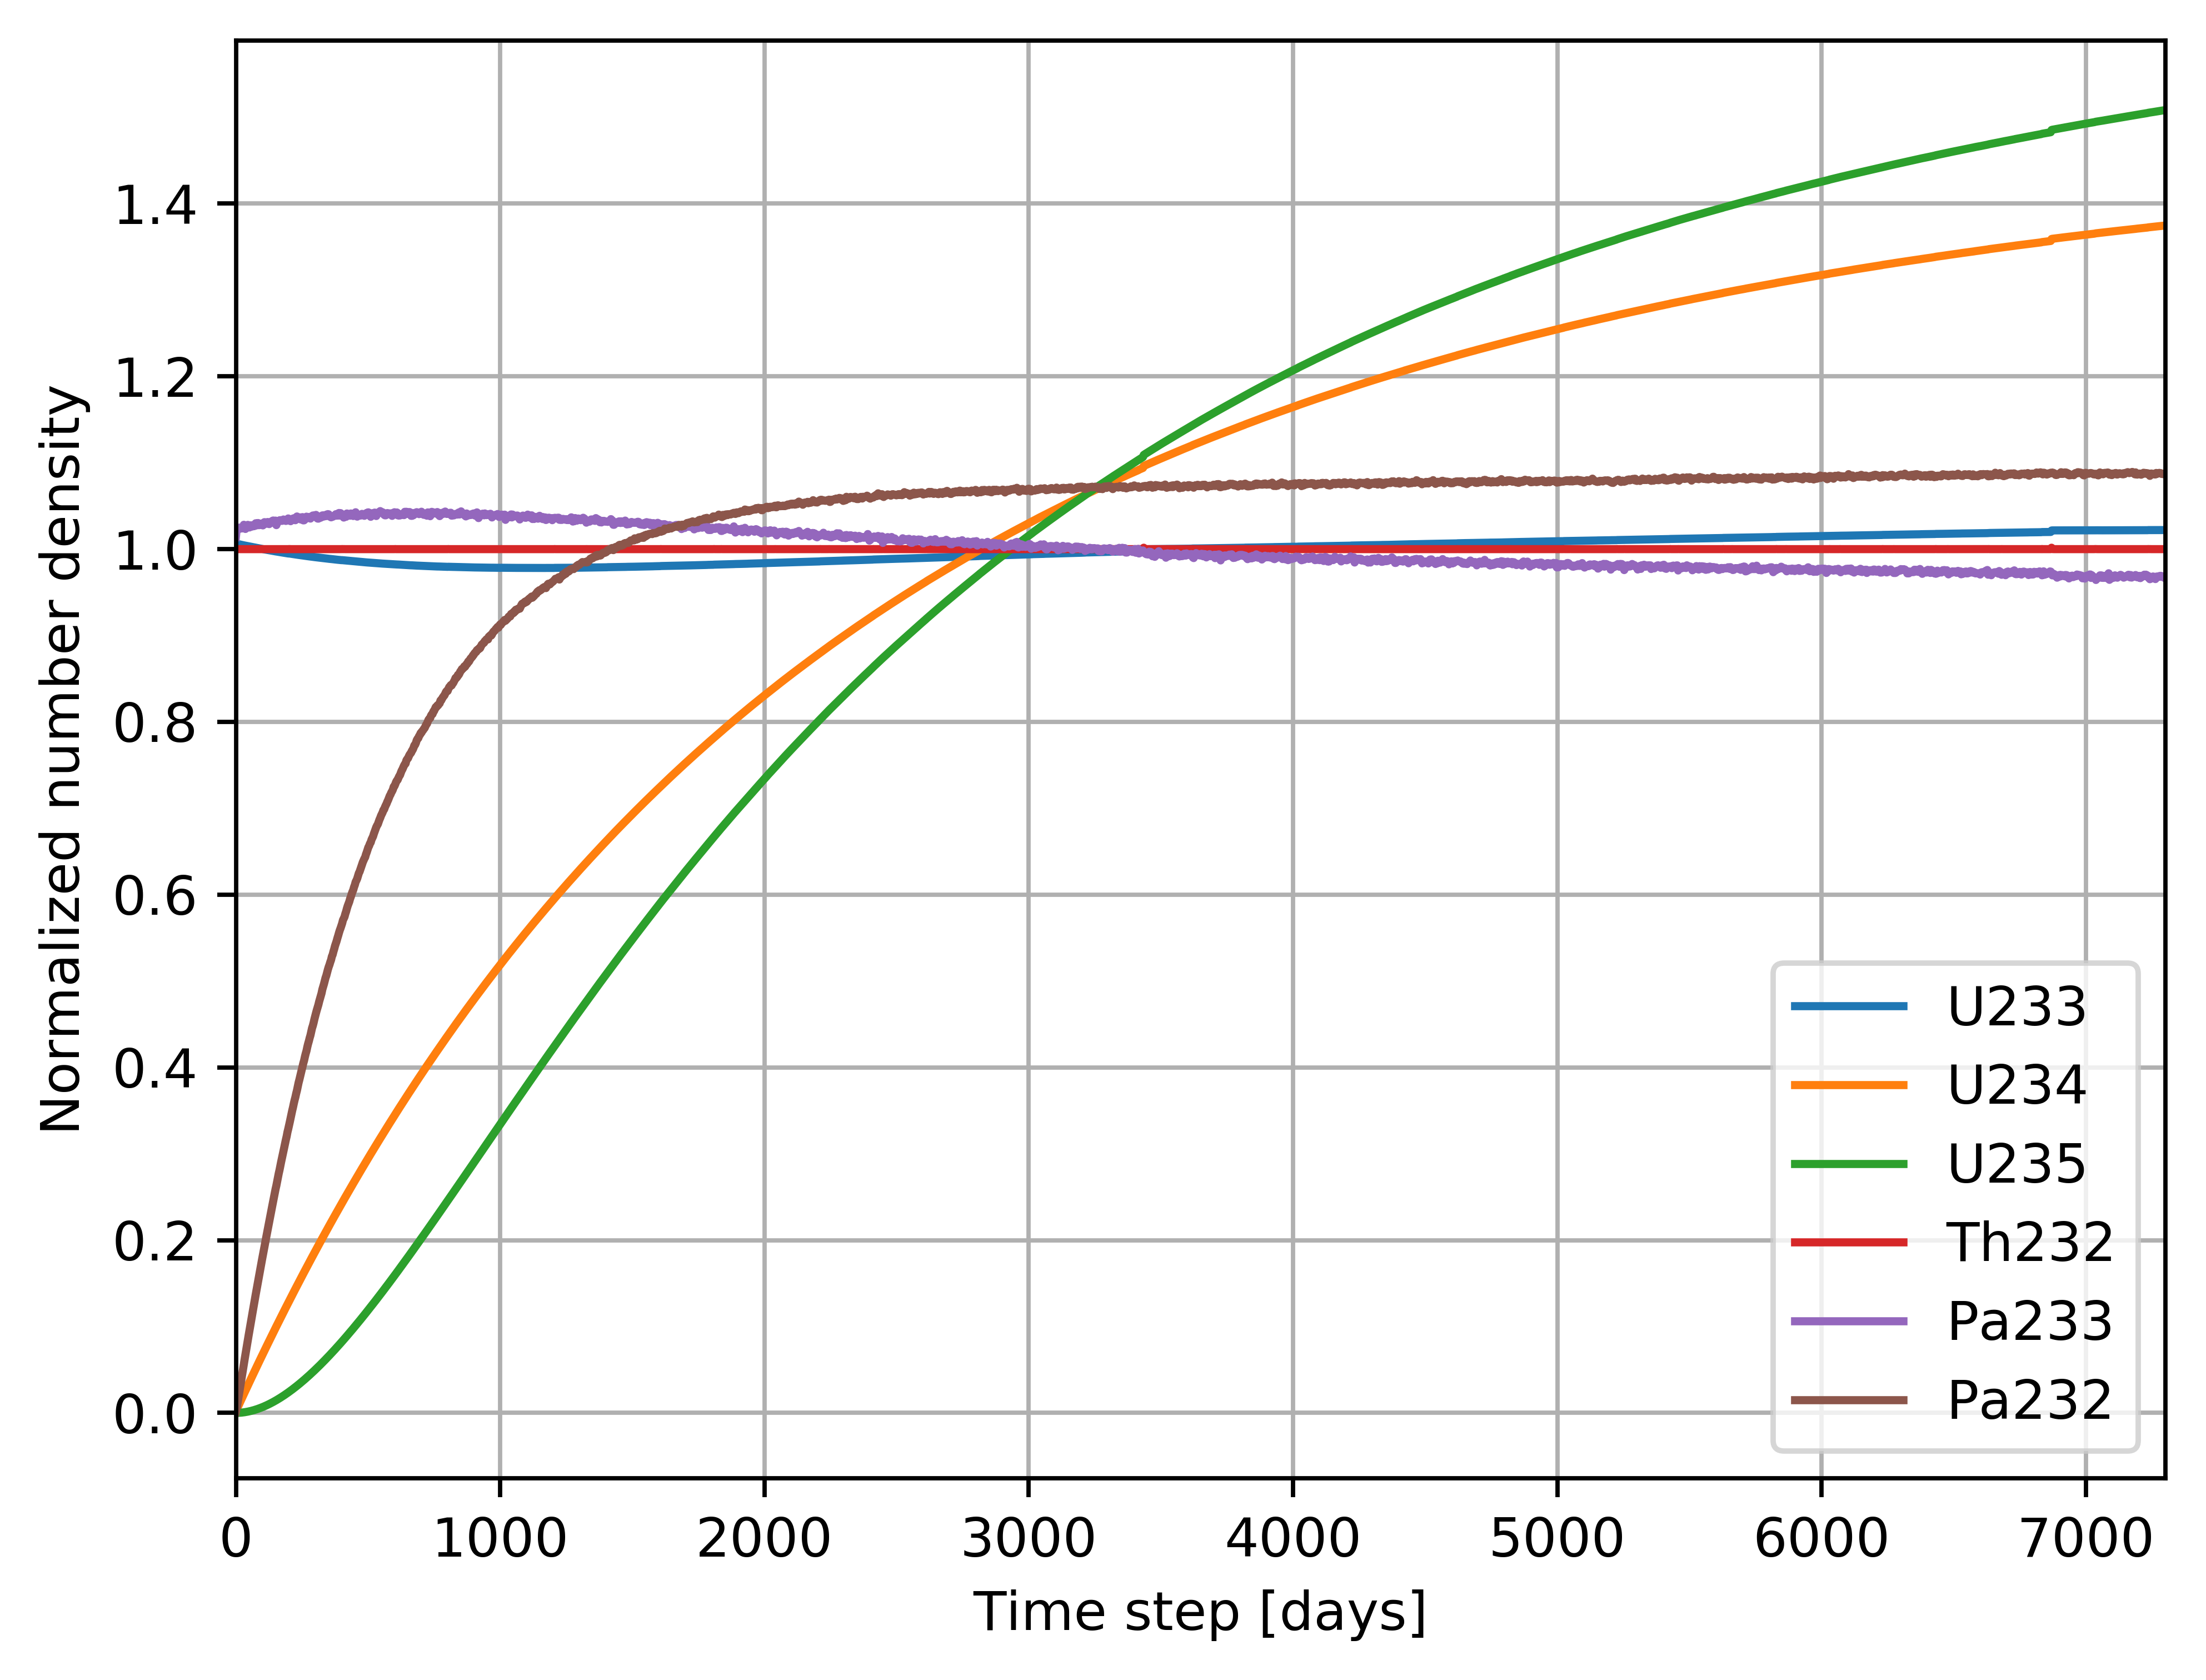
\includegraphics[width=1.05\textwidth]{major_isotopes_adens.png}
  \caption{Normalized number density of major nuclides during the reactor operation.}
  \vspace{-0.6em}
  \label{fig:adens_eq}
\end{figure}
\FloatBarrier

\begin{figure}[htp!] % replace 't' with 'b' to 
  \centering
  \vspace{-1.3em}
  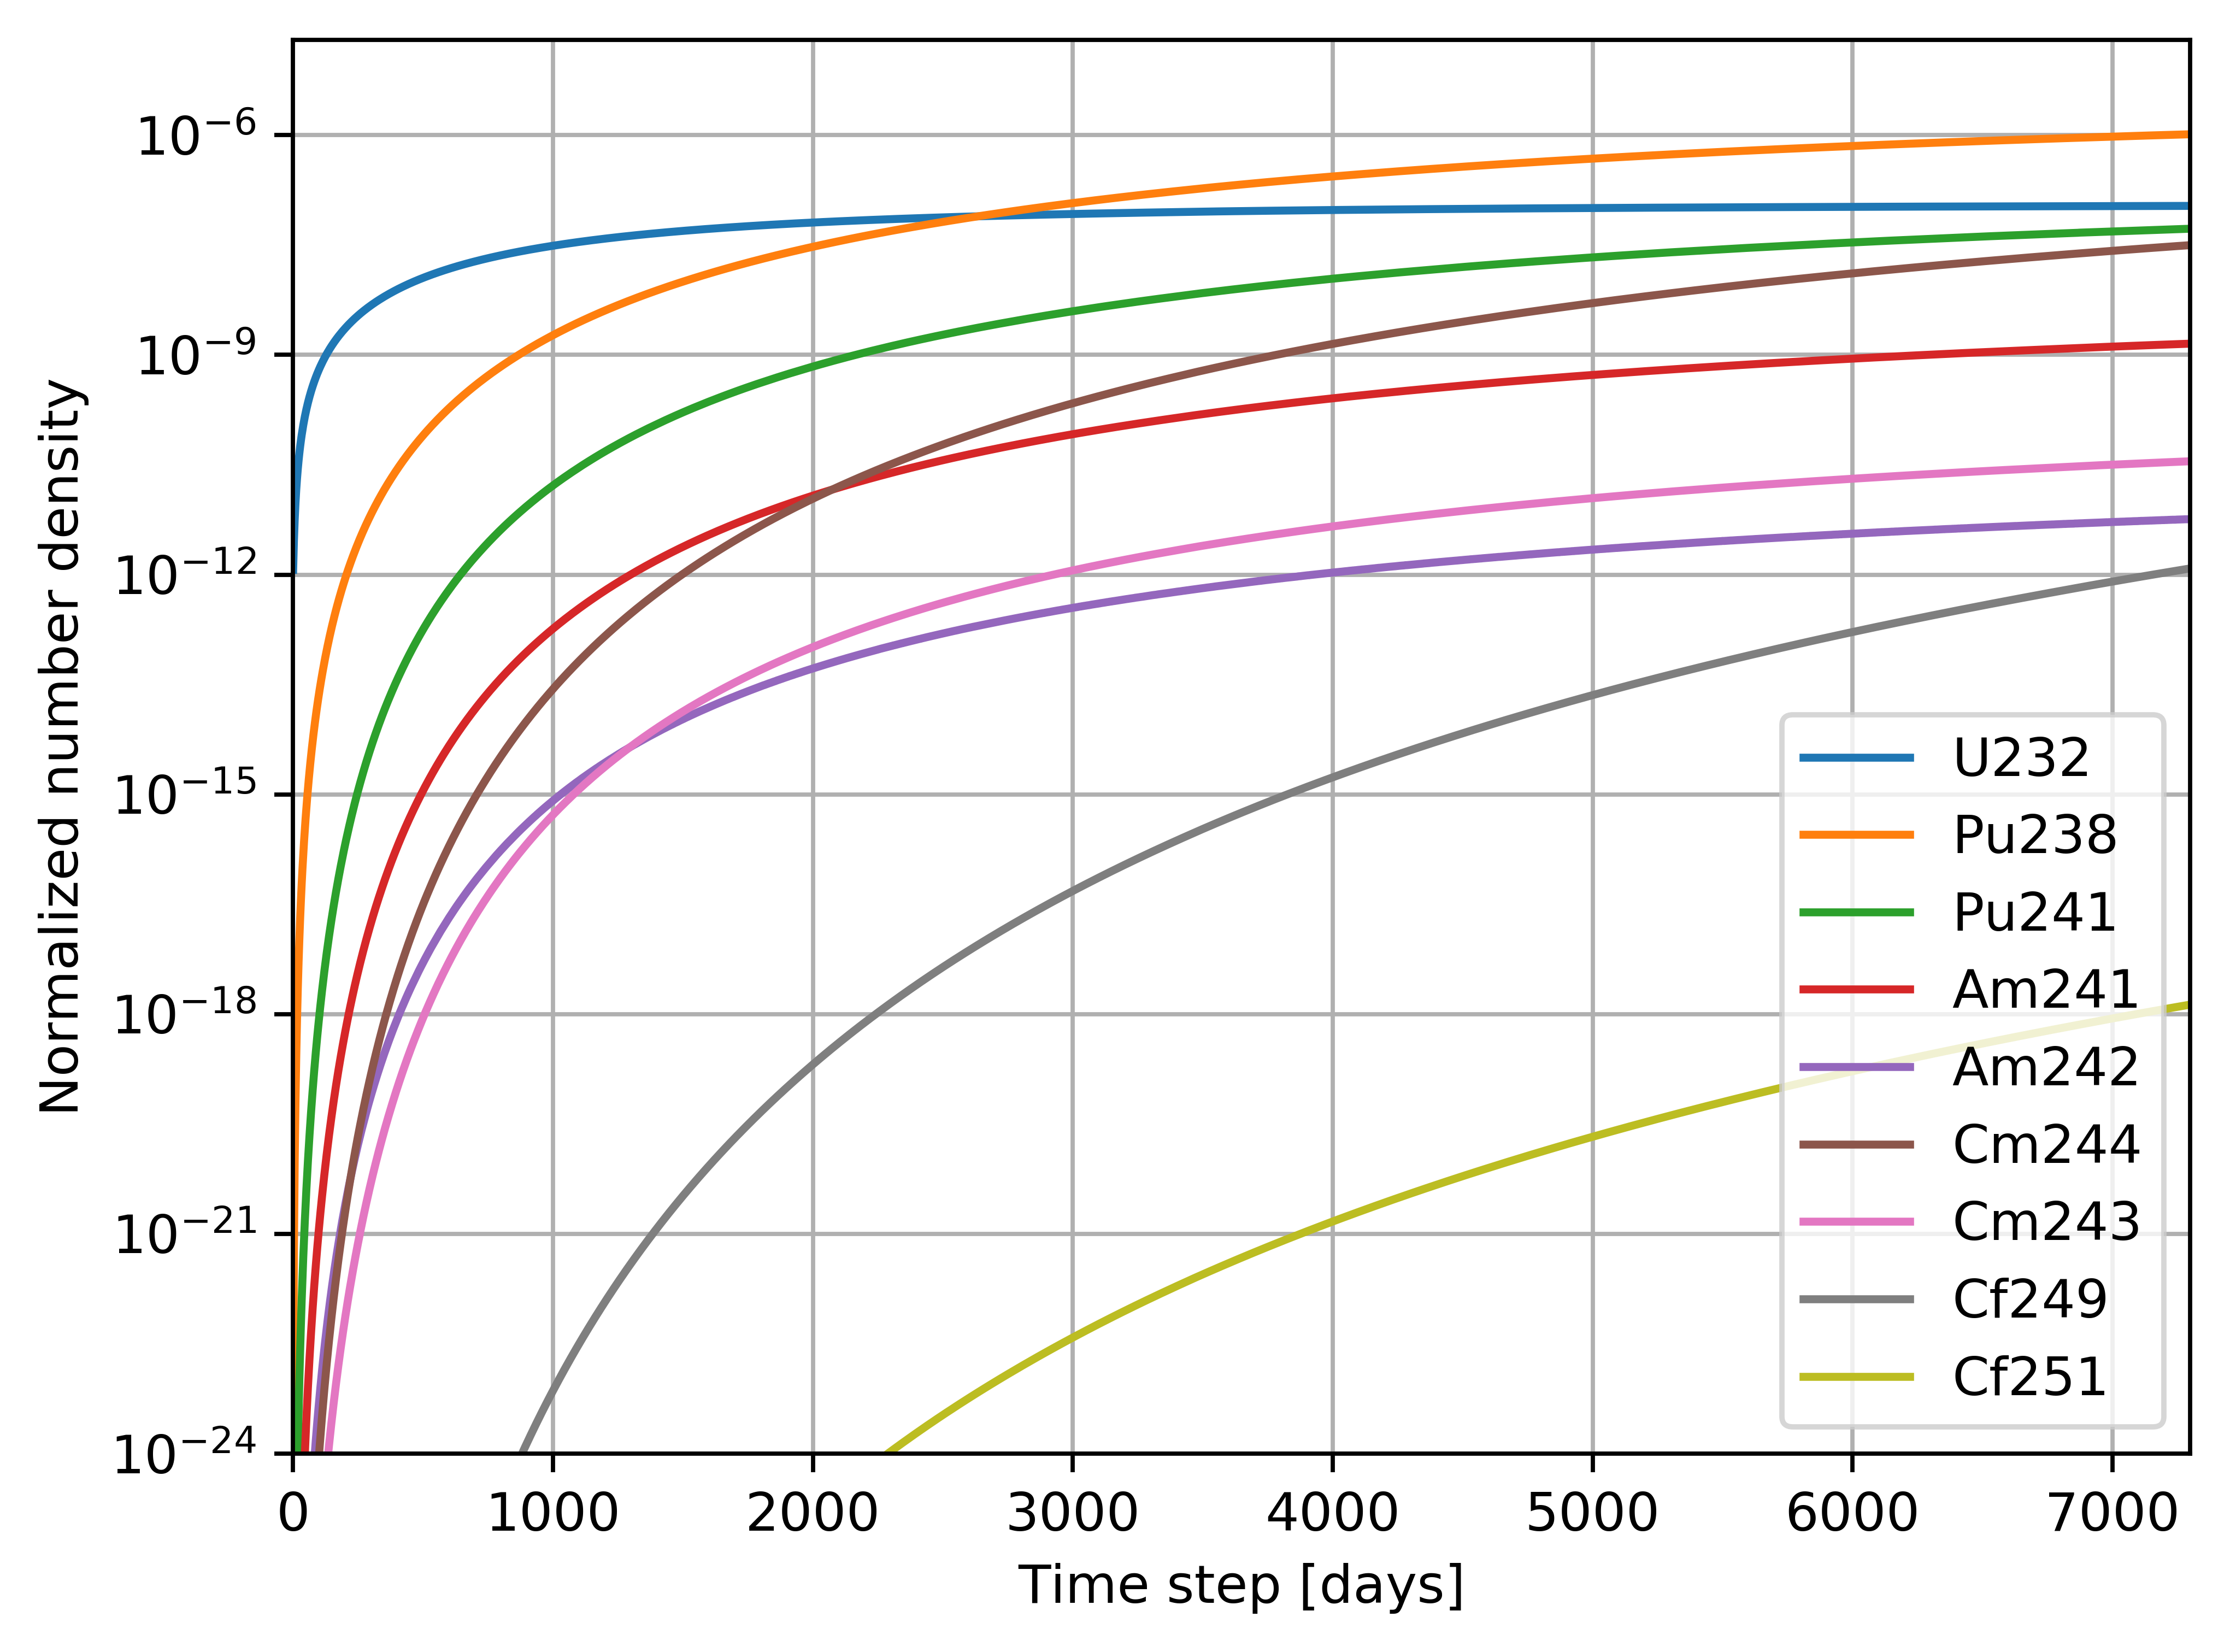
\includegraphics[width=\textwidth]{fissile_short.png}
   \vspace{-1.5em}
  \caption{Absolute number density of short-lived fissile nuclides ($\tau_{1/2}<900y$) during the reactor operation.}
  \vspace{-1.6em}
  \label{fig:fissile_short}
\end{figure}
\begin{figure}[hbp!] % replace 't' with 'b' to 
  \centering
  \vspace{-0.3em}
  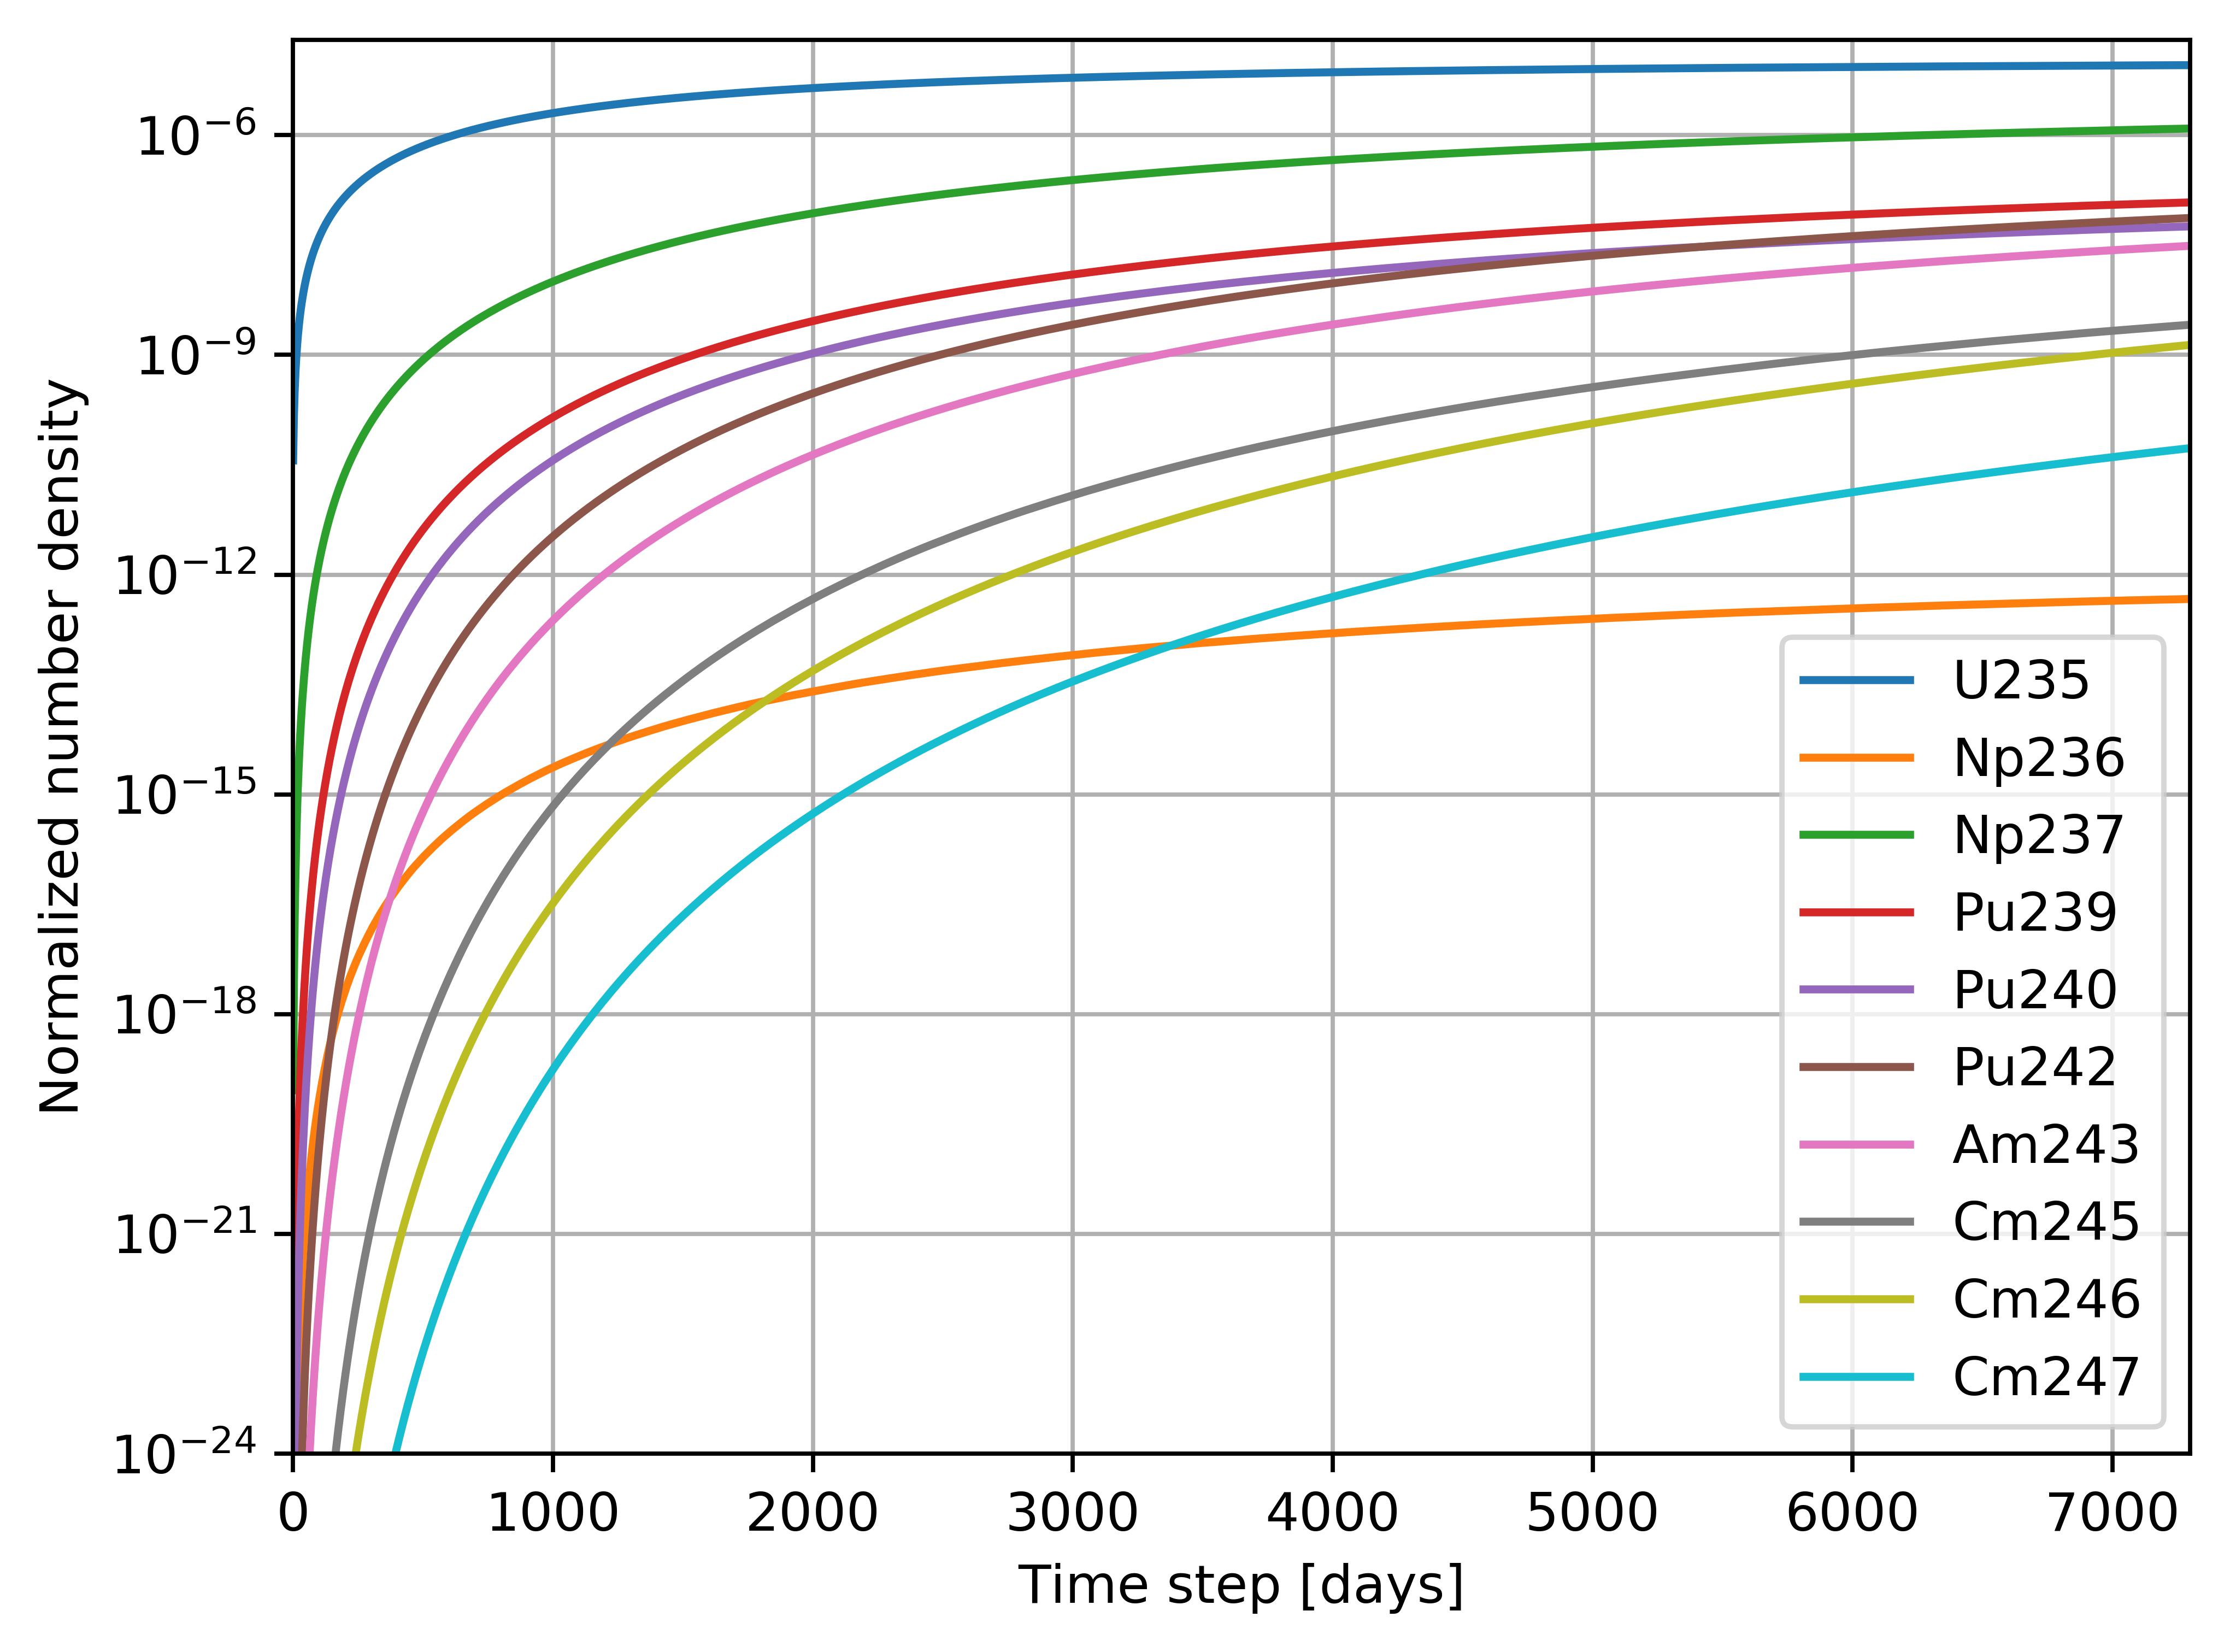
\includegraphics[width=\textwidth]{fissile_long.png}
   \vspace{-1.5em}
  \caption{Absolute number density of long-lived fissile nuclides ($\tau_{1/2}>900y$) during the reactor operation.}
  \vspace{-2.6em}
  \label{fig:fissile_long}
\end{figure}
\FloatBarrier

\section{Neutron spectrum}
Figure~\ref{fig:spectrum} shows the normalized neutron flux spectrum for the full-core \gls{MSBR} model in the energy range from $10^{-8}$ to $10$ MeV. The neutron energy spectrum for the full-core at equilibrium is harder than at startup due to $^{238}$Pu, $^{239}$Pu, $^{240}$Pu, $^{241}$Pu, and $^{242}$Pu accumulation in the core during reactor operation. 

\begin{figure}[htp!] % replace 't' with 'b' to force it to 
  \centering
    \vspace{-0.3em}
  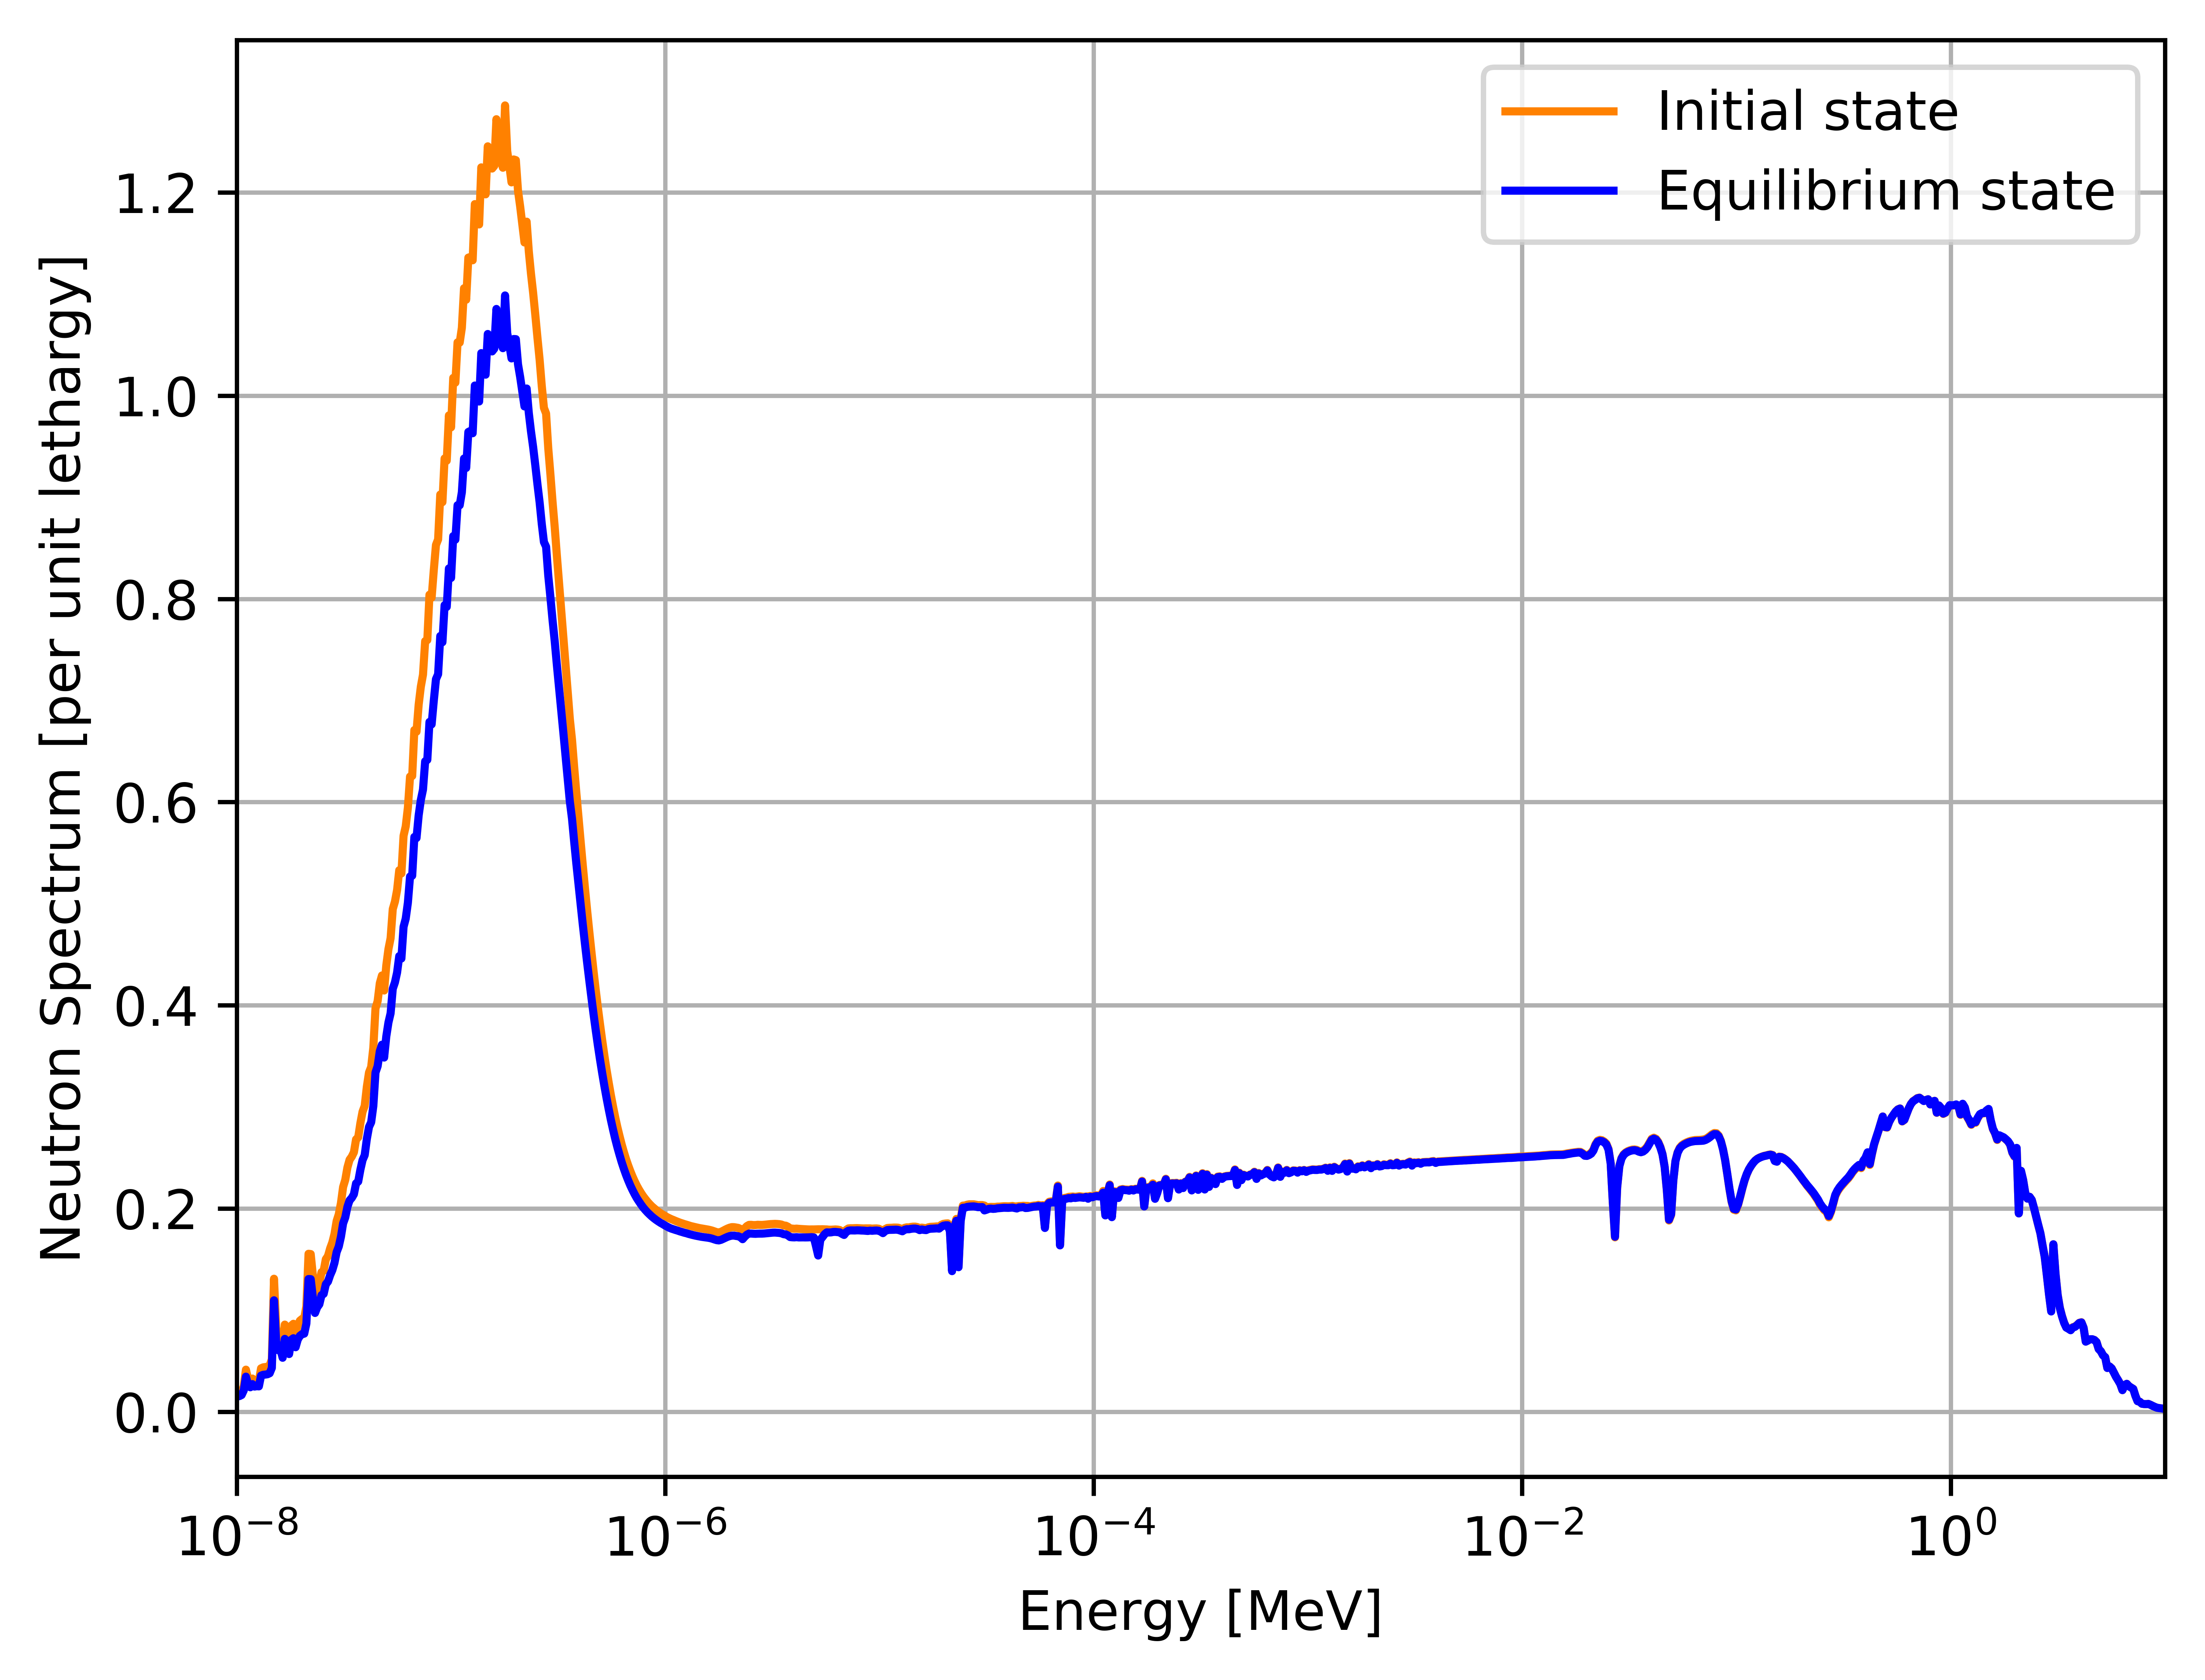
\includegraphics[width=1.05\textwidth]{spectrum.png} 
  \caption{Neutron flux energy spectrum normalized by unit lethargy for initial and equilibrium fuel salt composition.}
    \vspace{-0.6em}
  \label{fig:spectrum}
\end{figure}
\FloatBarrier

Figure~\ref{fig:spectrum_zones_init}, \ref{fig:spectrum_zones_eq} shows that zone I produced much more thermal neutrons than zone II, indicating that the majority of fissions occured in the central part of the core. In the undermoderated zone II, the neutron energy spectrum is harder which leads to more capture of neutrons by $^{232}$Th and helps a achieve relatively high breeding ratio. Moreover, the (n,$\gamma$) resonance energy range in $^{232}$Th is from 10$^{-4}$ to 10$^{-2}$ MeV. Therefore, the moderator-to-fuel ratio for zone II was chosen to shift the neutron energy spectrum in this range. Furthermore, in the central core region (zone I), the neutron energy spectrum shifts to a harder spectrum over 20 years of reactor operation. In contrast, in the outer core region (zone II) a similar spectral shift takes place at a reduced scale. This resuls is in a good agreement with original ORNL report \cite{robertson_conceptual_1971} and most recent whole-core steady-state study \cite{park_whole_2015}.

It is important to obtain the epithermal and thermal spectra to produce $^{233}$U from $^{232}$Th because the radiative capture cross section of thorium monotonically decreases from $10^{-10}$ MeV to $10^{-5}$ MeV. Hardening the spectrum tends to significantly increase resonance absorption in thorium and decrease the absorptions in fissile and construction materials. Thus, a signficant amount fissile material will be needed to make the reactor critical. 

\begin{figure}[htp!] % replace 't' with 'b' to force it to 
  \centering
    \vspace{-0.3em}
  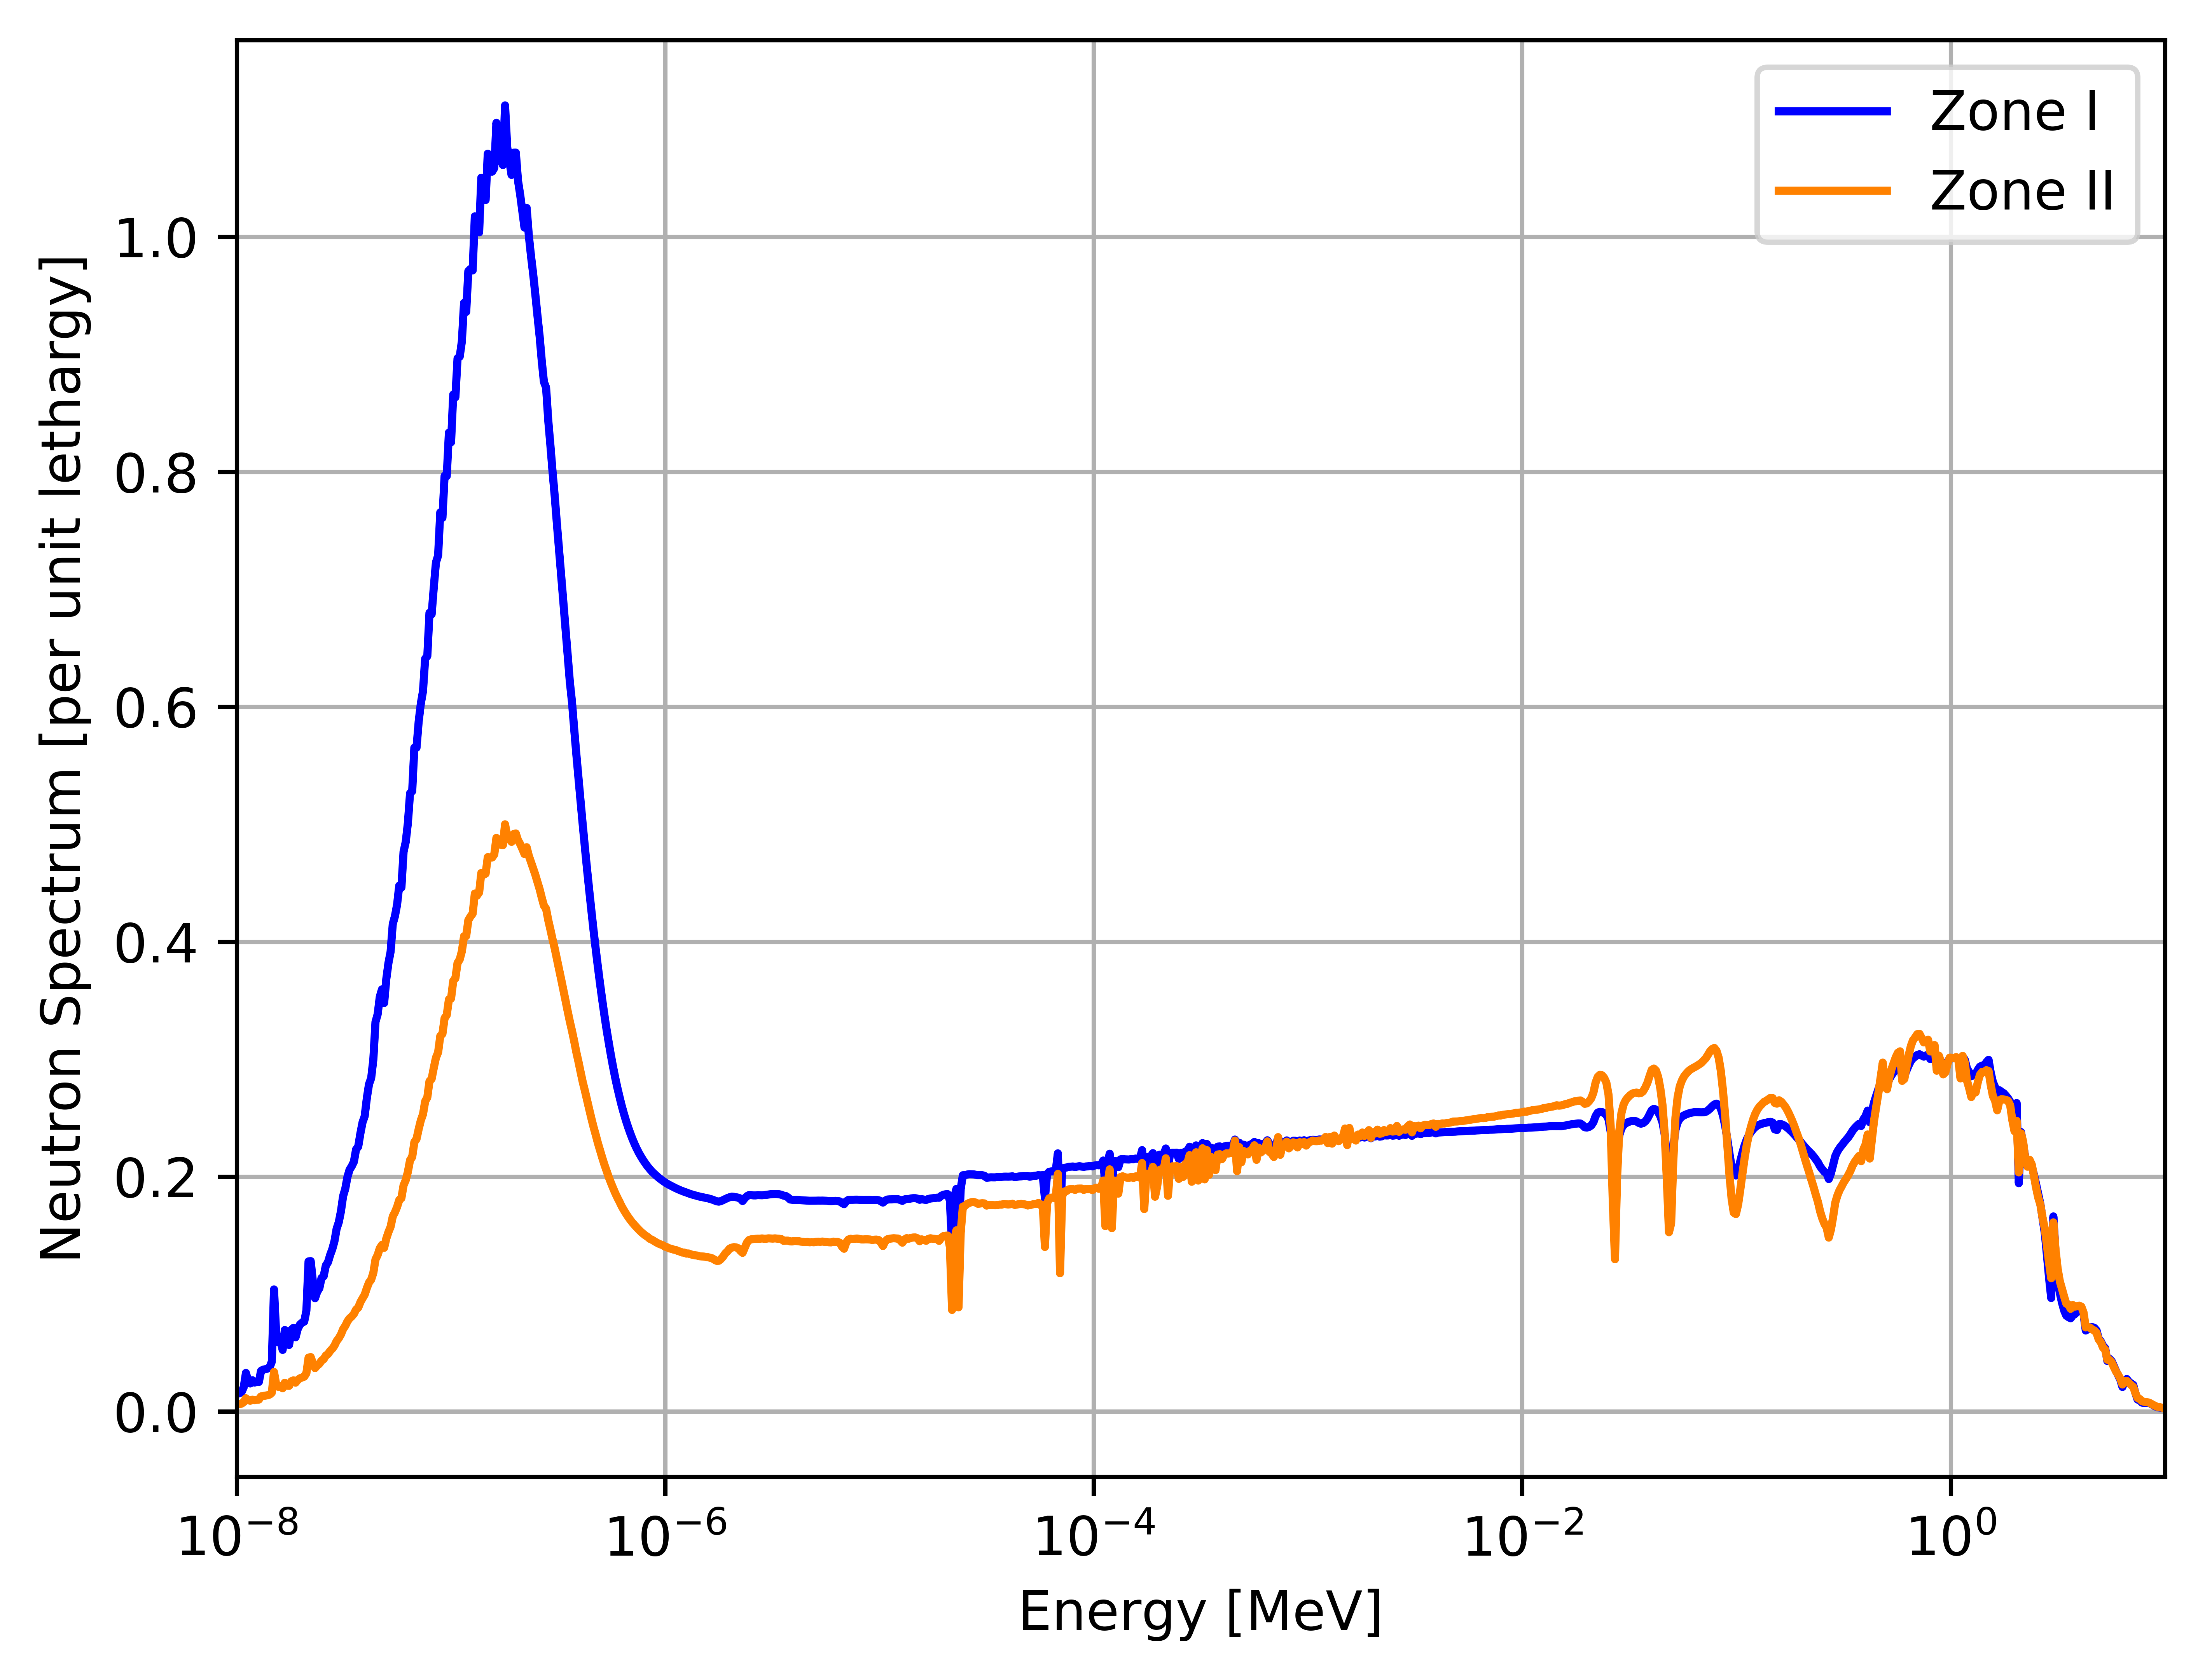
\includegraphics[width=1.05\textwidth]{spectrum_zones_init.png} 
  \caption{Neutron flux energy spectrum in different core regions normalized by unit lethargy for the initial fuel salt composition.}
    \vspace{-1.6em}
  \label{fig:spectrum_zones_init}
\end{figure}
\begin{figure}[htp!] % replace 't' with 'b' to force it to 
  \centering
    \vspace{-0.3em}
  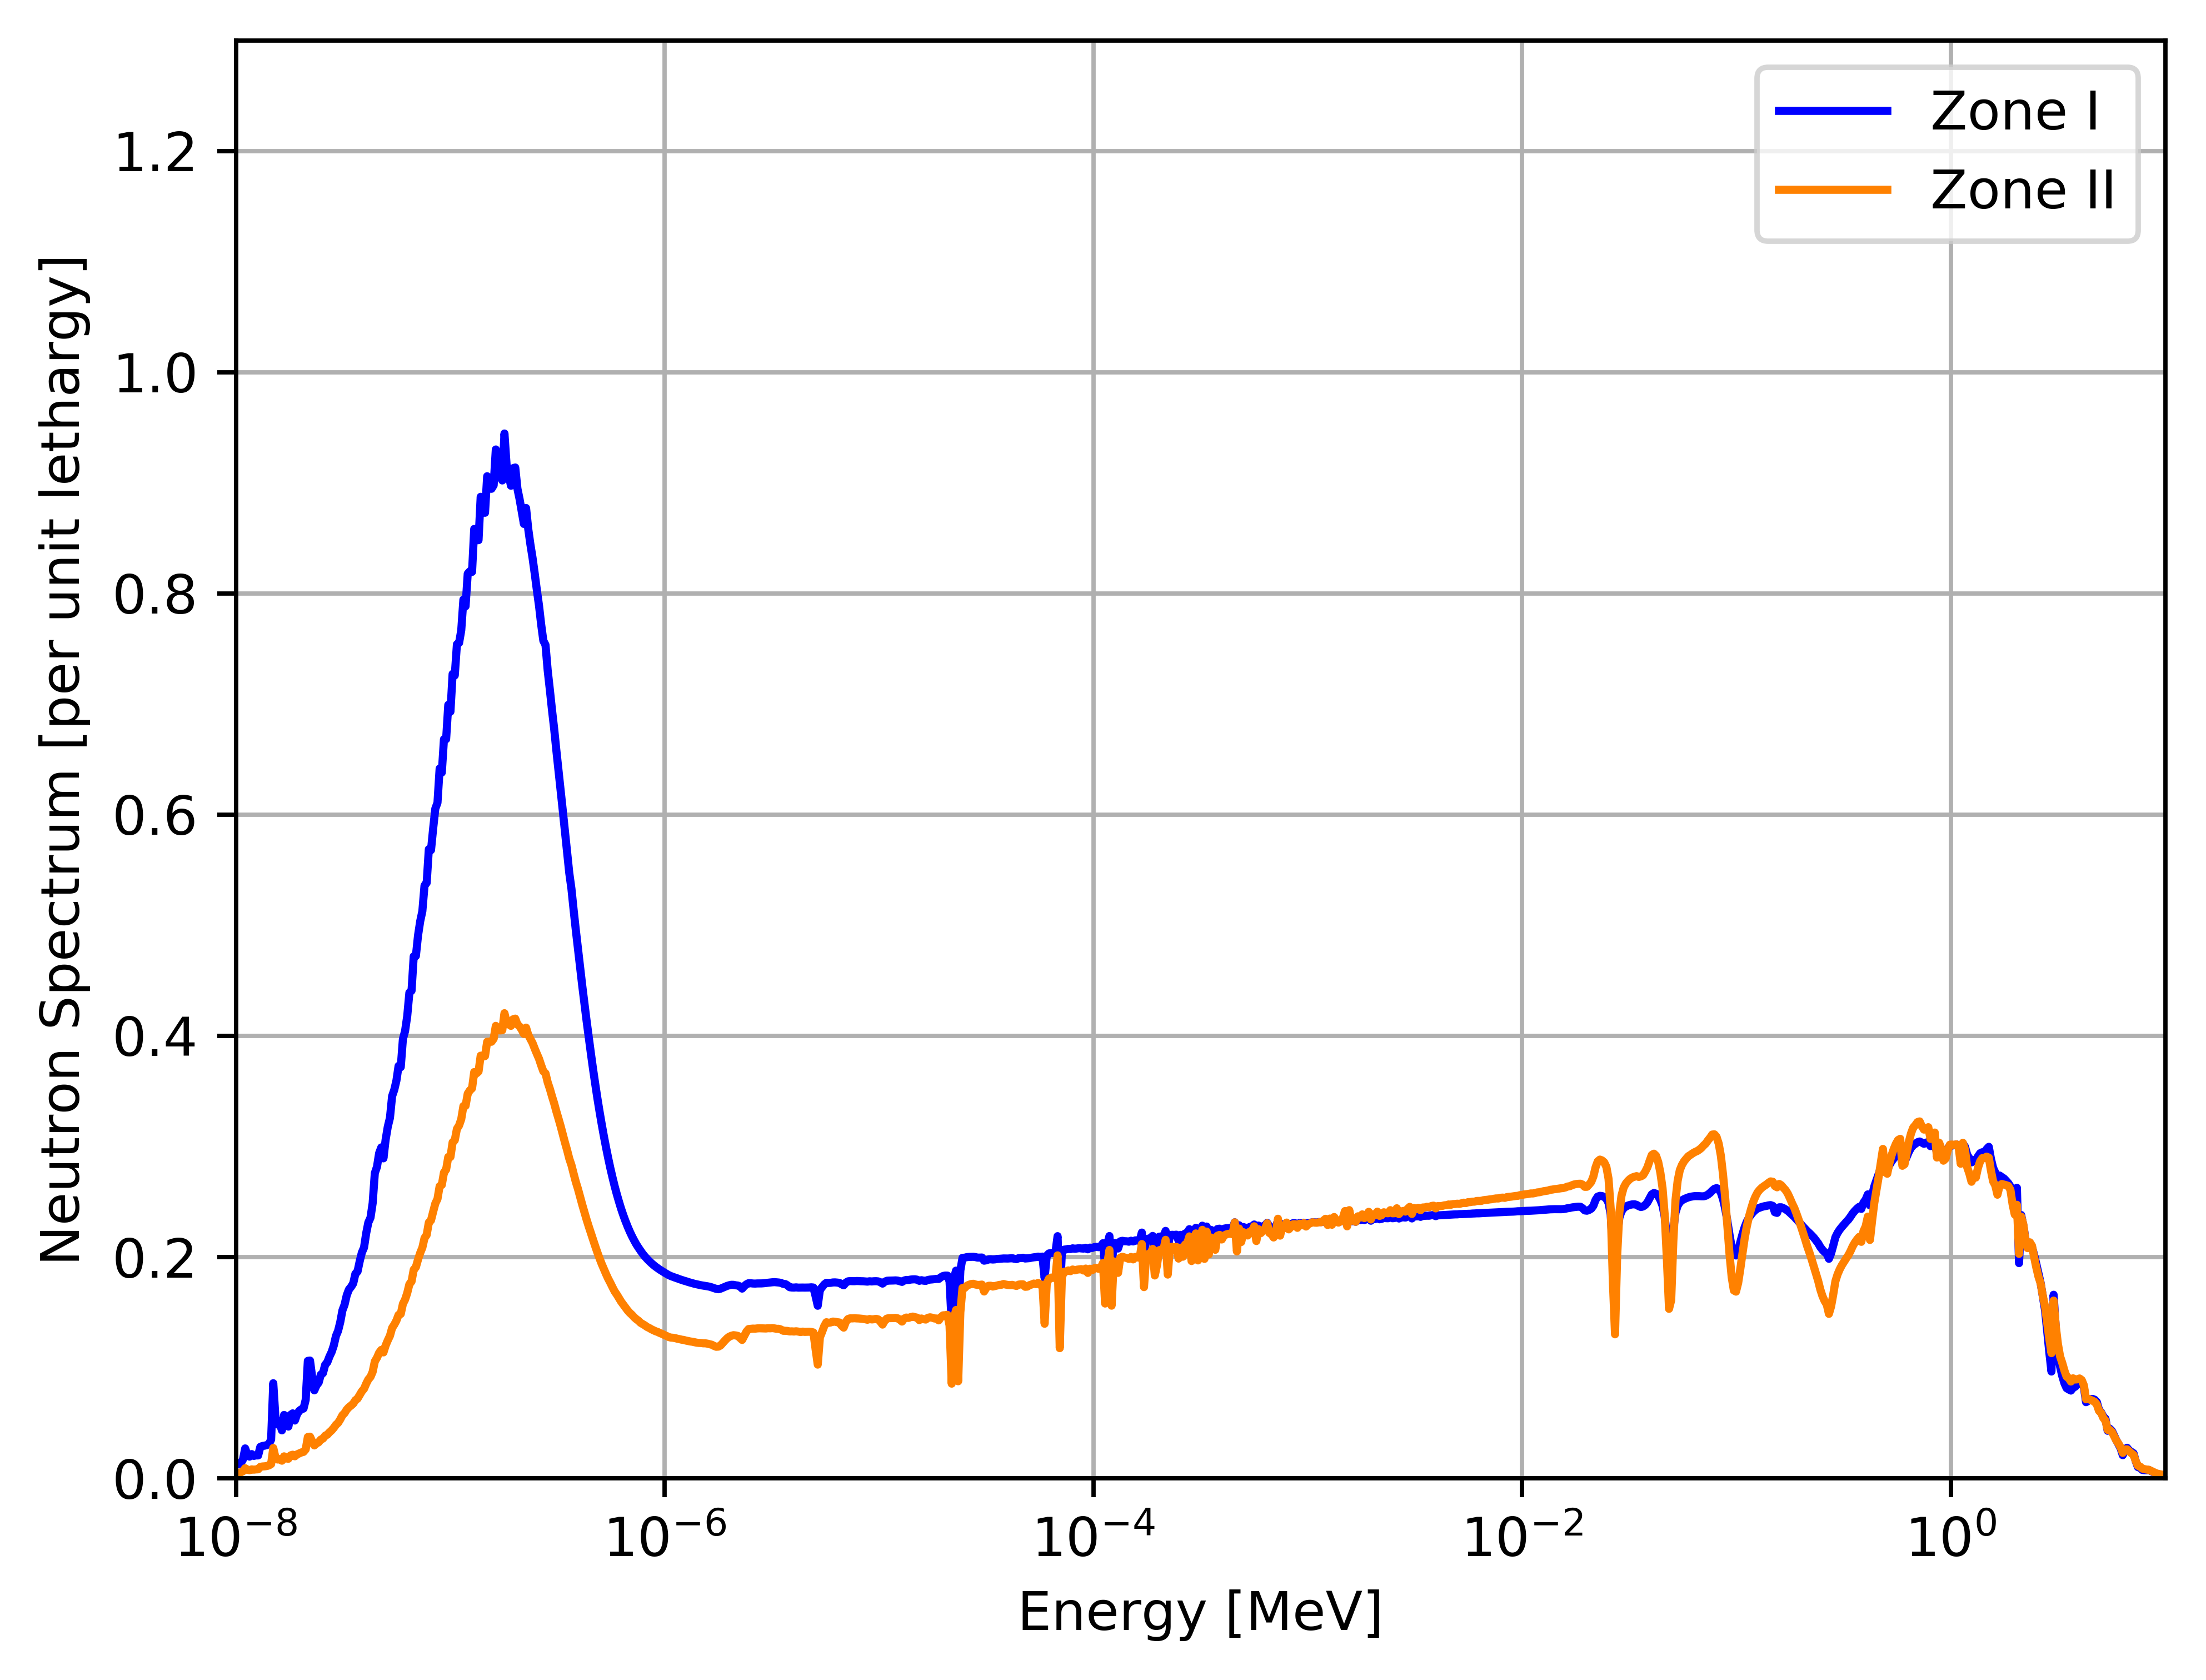
\includegraphics[width=1.05\textwidth]{spectrum_zones_eq.png} 
  \caption{Neutron flux energy spectrum in different core regions normalized by unit lethargy for the equilibrium fuel salt composition.}
    \vspace{-1.6em}
  \label{fig:spectrum_zones_eq}
\end{figure}
\FloatBarrier

\section{Neutron flux}
Figure~\ref{fig:radial_flux} shows the radial distribution of fast and thermal neutron flux for both initial and equilibrium composition. The neutron flux has the same shape for both compositions but the equilibrium case has a harder spectrum. A significant spectral shift was observed for the central region of the core (zone I) when for the outer region (zone II) it is neglectable for fast but notable for thermal neutrons. This neutron flux radial distribution is in a good agreement with original ORNL report \cite{robertson_conceptual_1971}. On the whole, spectrum hardening during \gls{MSBR} operation should be carefully studied for designing the reactivity control system.

\begin{figure}[htp!] % replace 't' with 'b' to force it to 
  \centering
    \vspace{-0.3em}
  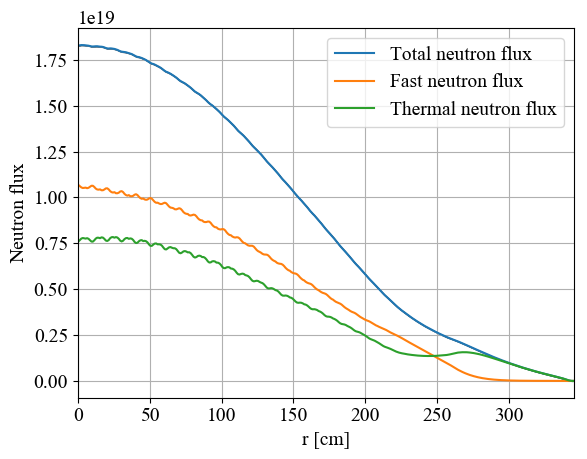
\includegraphics[width=1.05\textwidth]{radial_flux.png} 
  \caption{Radial neutron flux distribution for initial and equilibrium fuel salt composition.}
    \vspace{-0.6em}
  \label{fig:radial_flux}
\end{figure}
\FloatBarrier

\section{Power and breeding distribution}
Table~\ref{tab:powgen_fraction} shows the power fraction in each zone for initial and equilibrium fuel composition. Figure~\ref{fig:pow_den} demonstrates the normalized power distribution of the \gls{MSBR} one-fourth core at both states. For both the initial and equilibrium compositions, fission primarly occurs in the center of the core, namely zone I. The spectral shift during reactor operation results in different power fractions at startup and equilibrium, but most of the power is still generated in zone I. Figure~\ref{fig:breeding_den} shows the neutron capture reaction rate distribution for $^{232}$Th normalized by the total neutron flux for initial and equilibrium states. The distribution reflects the spatial distribution of $^{233}$Th production in the core. The thorium-232 then $\beta$-decays to $^{233}$Pa which is the precursor for $^{233}$U production. Accordingly, this characteristic represents the breeding distribution in the \gls{MSBR} core. Spectral shift does not cause significant changes in power nor in breeding distribution. Even after 20 years of operation, most of the power still is generated in zone I though the majority of $^{233}$Th is produced in zone II which is in a good agreement with original ORNL report \cite{robertson_conceptual_1971}.

%%%%%%%%%%%%%%%%%%%%%%%%%%%%%%%%%%%%%%%%
\begin{table}[ht!]
  \centering
  \caption{Power generation fraction in each zone for initial and equilibrium state.}
\begin{tabular}{| m{0.22\textwidth} | m{0.22\textwidth} | m{0.22\textwidth} |} \hline
Core region      & Initial      & Equilibrium   \\ [3pt]\hline   
Zone I           & 97.91\%      & 98.12\%   \\ [3pt] \hline
Zone II          & 2.09\%       & 1.88\%   \\ [3pt] \hline
\end{tabular}
  \label{tab:powgen_fraction}
\end{table}
%%%%%%%%%%%%%%%%%%%%%%%%%%%%%%%%%%%%%%%%%%%%%%%%%%%%%%%%%%%%%%%%%%%%%%%%%%%%%%%%

\begin{figure}[htp!] % replace 't' with 'b' to force it to 
  \centering
    \vspace{-0.3em}
  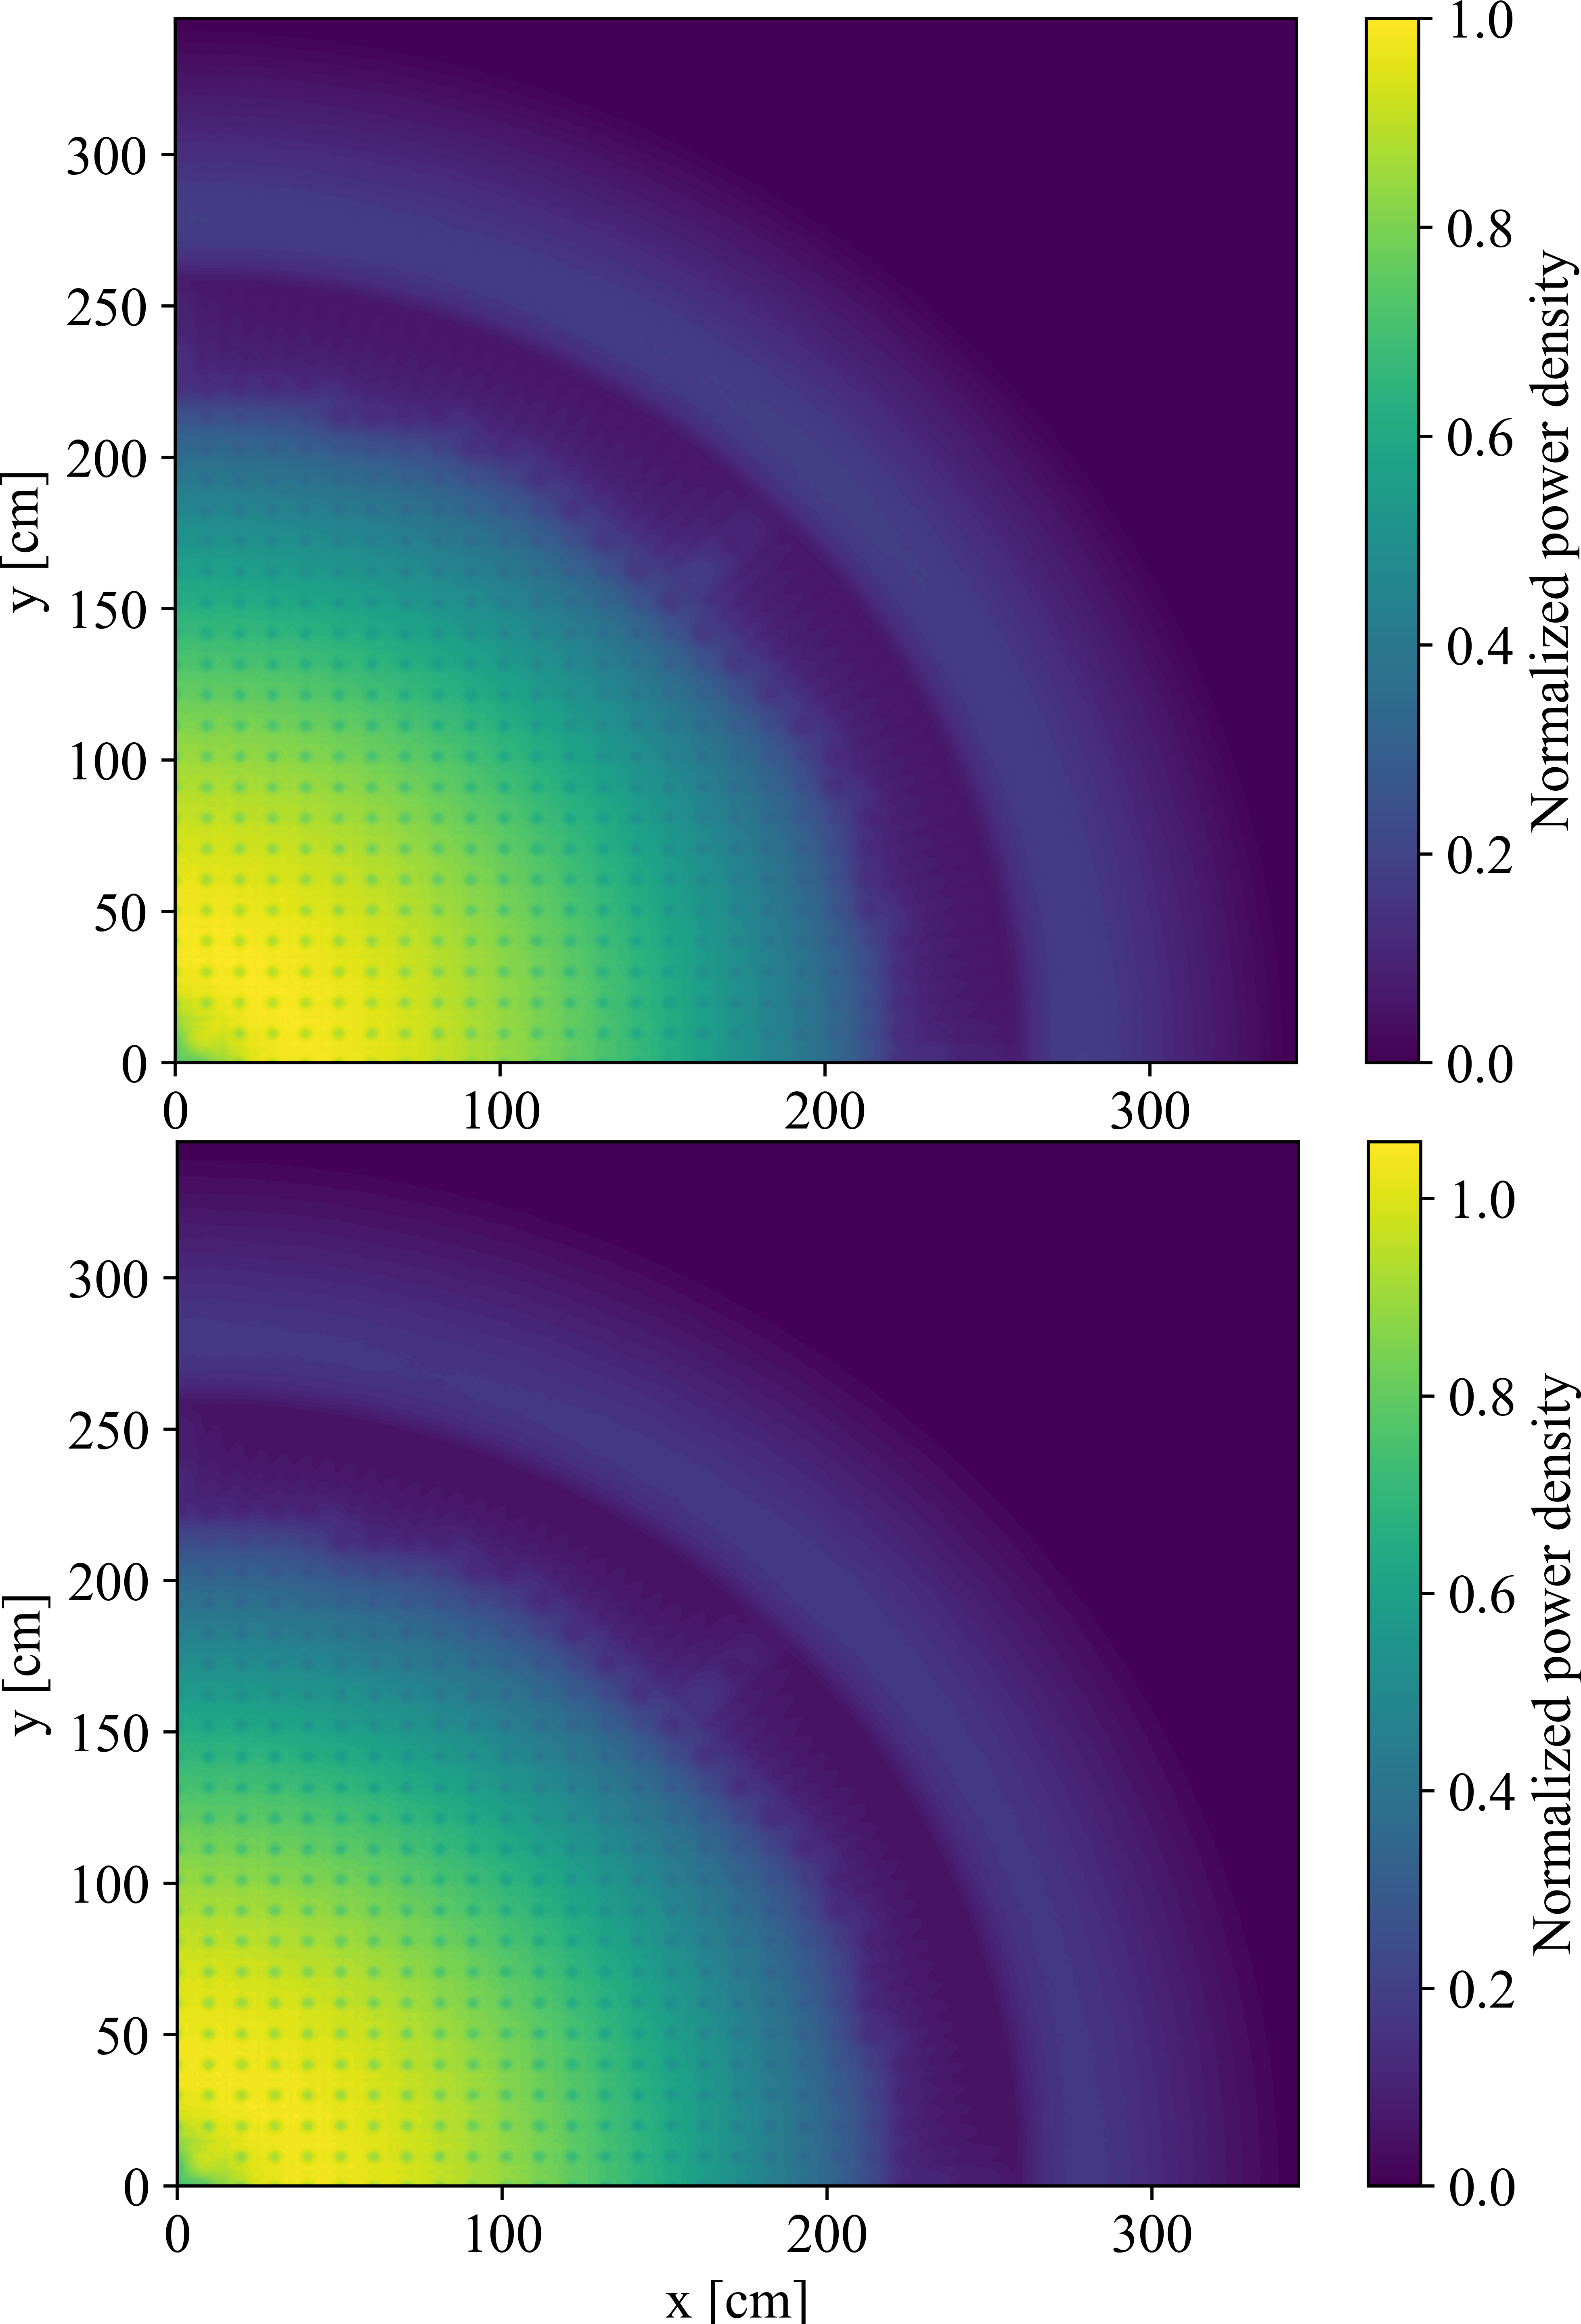
\includegraphics[width=1.05\textwidth]{power_distribution.png} 
  \caption{Normalized power density for initial (top) and equilibrium (bottom) fuel salt composition.}
    \vspace{-0.6em}
  \label{fig:pow_den}
\end{figure}
\FloatBarrier

\begin{figure}[htp!] % replace 't' with 'b' to force it to 
  \centering
    \vspace{-0.3em}
  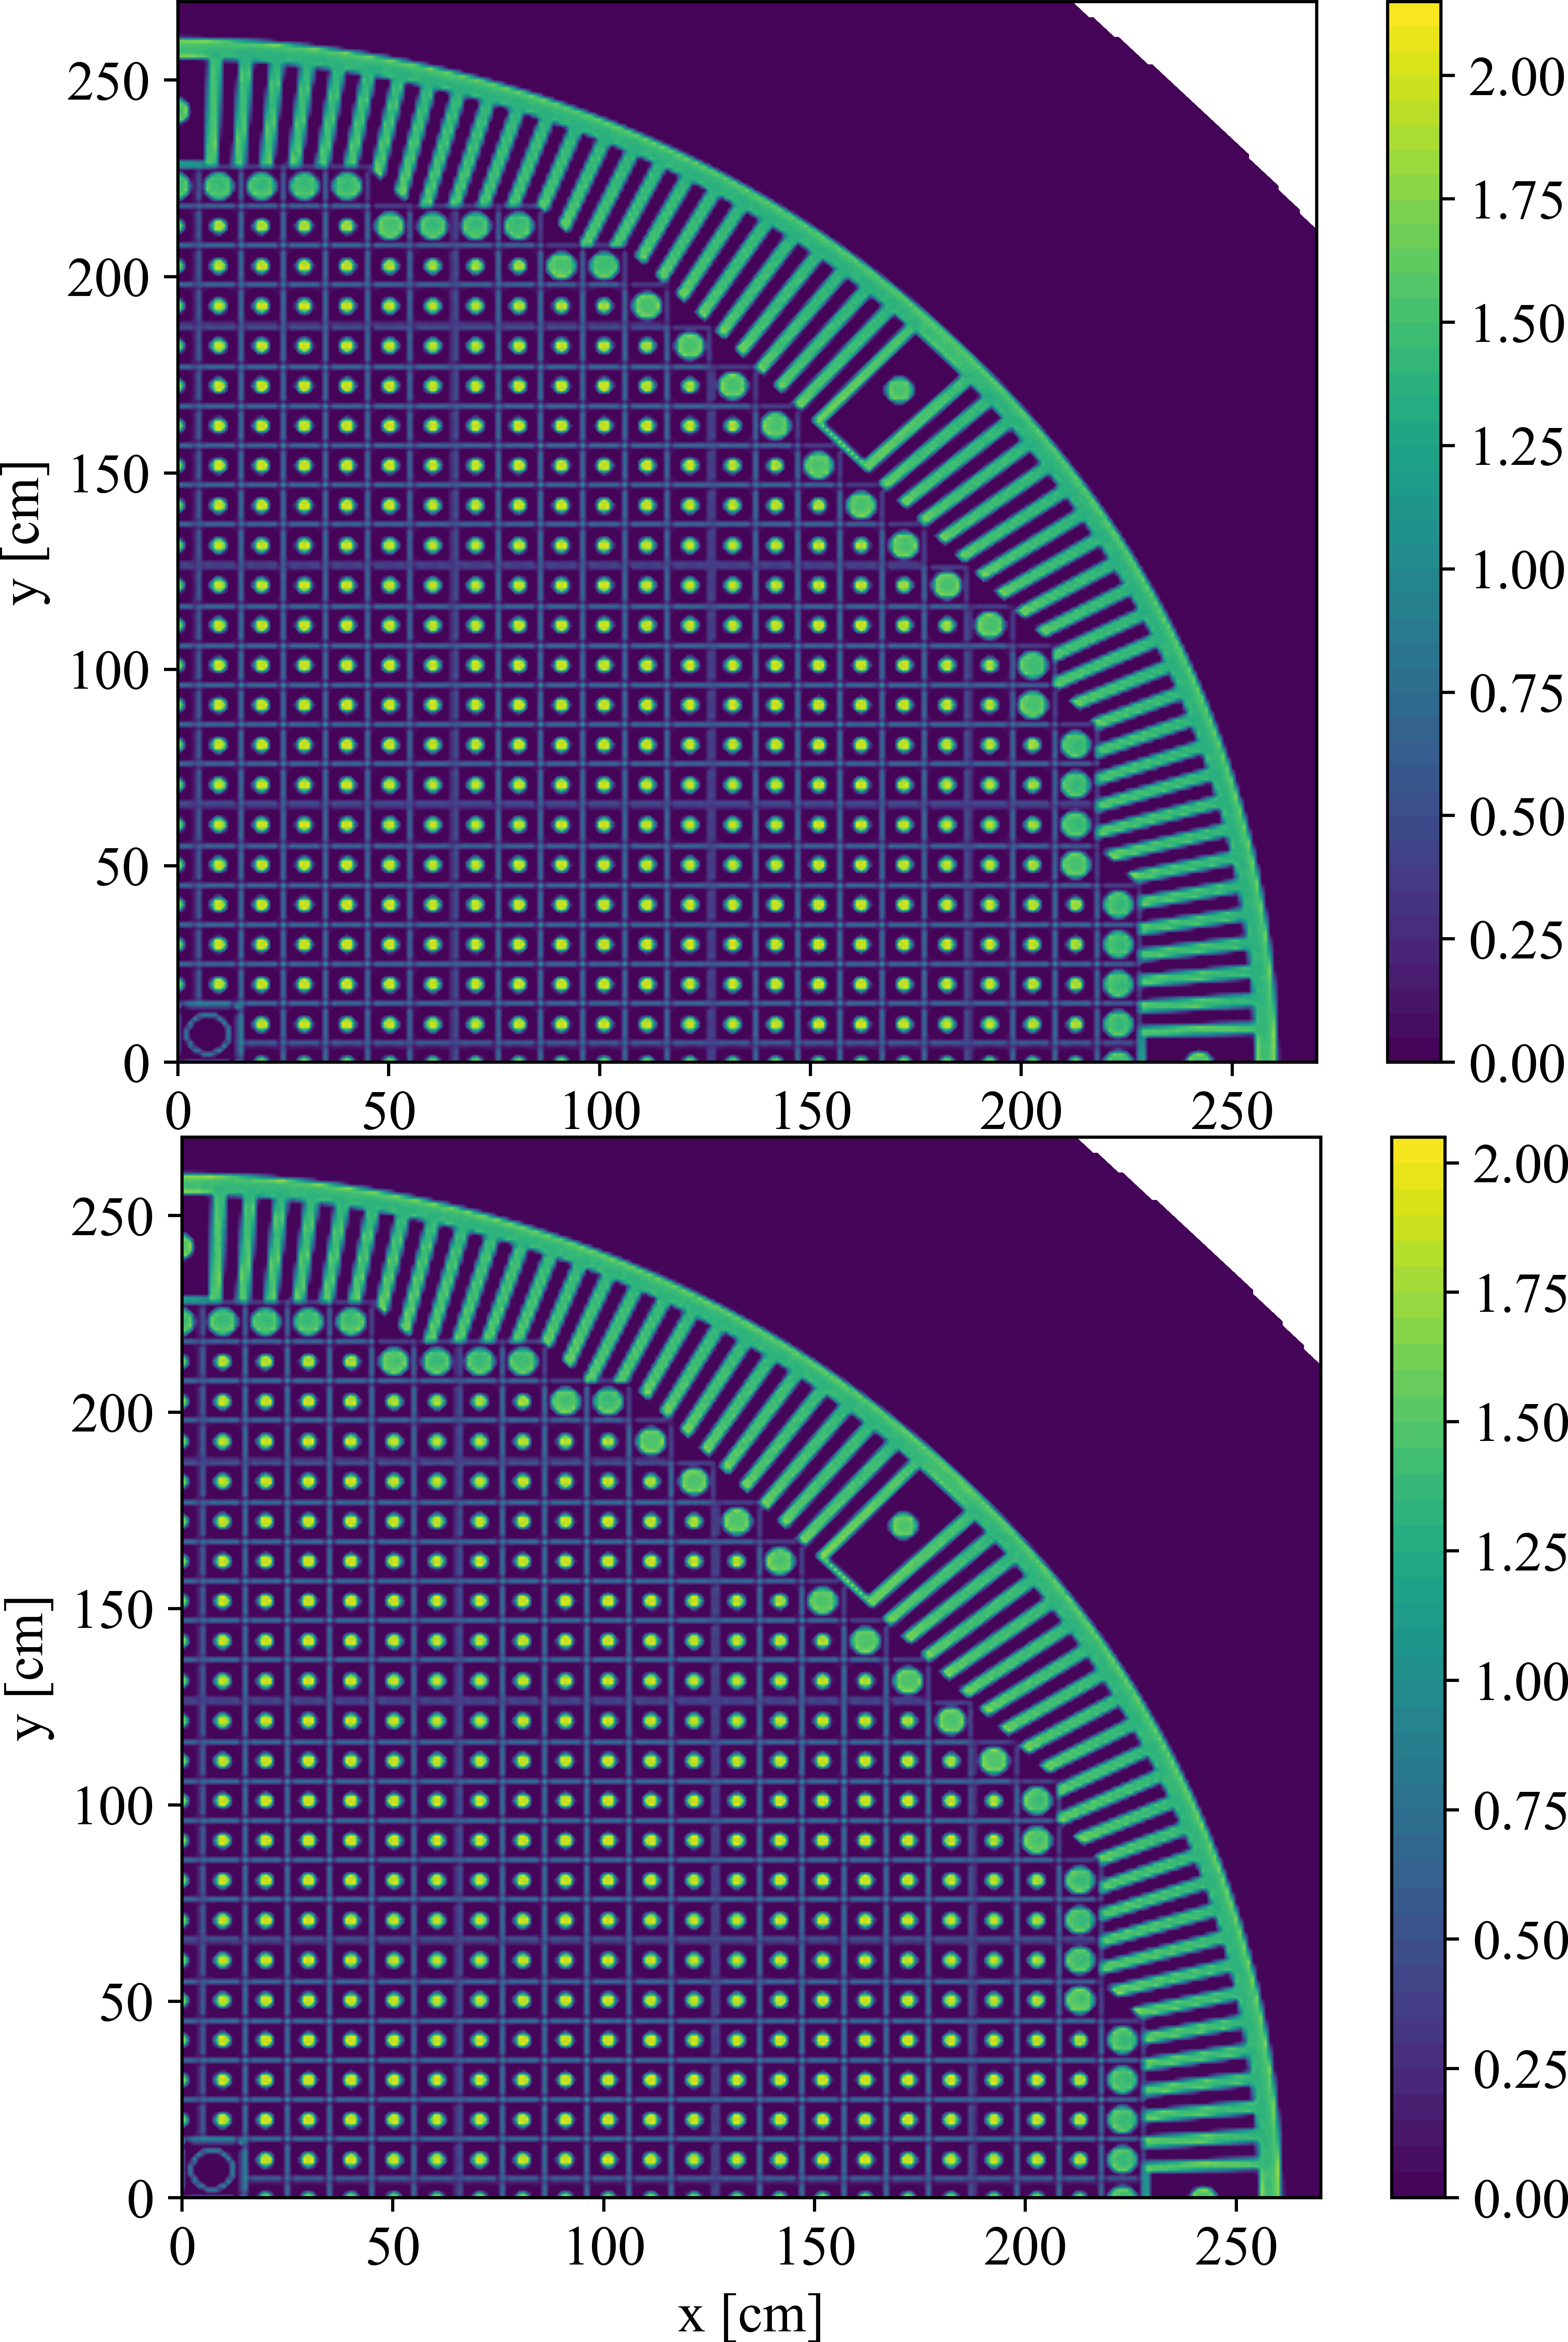
\includegraphics[width=1.05\textwidth]{breeding_distribution.png} 
  \caption{$^{232}$Th neutron capture reaction rate normalized by total flux for initial (top) and equilibrium (bottom) fuel salt composition.}
    \vspace{-0.6em}
  \label{fig:breeding_den}
\end{figure}
\FloatBarrier

\section{Temperature coefficient of reactivity}
Table~\ref{tab:tcoef} summarizes temperature effects on reactivity calculated in this work for both initial and equilibrium fuel composition, and compared with original \gls{ORNL} report data \cite{robertson_conceptual_1971}. Uncertainty for each temperature coefficient also appears in Table~\ref{tab:tcoef}. The main physical principle underlying the reactor temperature feedback is an expansion of matter when it is heated. When the fuel salt temperature increases, the density of the salt decreases, but at the same time, the total volume of fuel salt in the core remains constant because it is bounded by the graphite. When the reactor graphite temperature grows, the density of graphite declines creating additional space for fuel salt. To determine temperature coefficients, the cross-section temperatures for fuel and moderator were changed from 900K to 1000K. Three different cases were considered:
\begin{enumerate}
  \item Temperature of fuel salt rising from 900K to 1000K.
  \item Temperature of graphite rising from 900K to 1000K.
  \item Whole reactor temperature rising from 900K to 1000K.
\end{enumerate}

%%%%%%%%%%%%%%%%%%%%%%%%%%%%%%%%%%%%%%%%
\begin{table}[ht!]
  \centering
  \caption{Temperature coefficients of reactivity for initial and equilibrium state.}
\begin{tabular}{| m{0.22\textwidth} | m{0.22\textwidth} | m{0.22\textwidth} | m{0.22\textwidth} |} \hline
   Reactivity coefficient [pcm/K]  & Initial      & Equilibrium  & Reference \cite{robertson_conceptual_1971} \\ [5pt]\hline   
Fuel salt        & $-3.22\pm0.044$ & $-1.53\pm0.046$ & $-3.22$  \\ [3pt] \hline
Moderator        & $+1.61\pm0.044$ & $+0.97\pm0.046$ & $+2.35$  \\ [3pt] \hline
Total            & $-3.1\pm0.04$   & $-0.97\pm0.046$ & $-0.87$  \\ [3pt] \hline
\end{tabular}
  \label{tab:tcoef}
\end{table}
%%%%%%%%%%%%%%%%%%%%%%%%%%%%%%%%%%%%%%%%%%%%%%%%%%%%%%%%%%%%%%%%%%%%%%%%%%%%%%%%
In the first case, changes in the fuel temperature only impact fuel density. In this case, the geometry is unchanged because the fuel is a liquid. However, when the moderator heats up, both the density and the geometry change due to thermal 
expansion of the solid graphite blocks and reflector. Accordingly, the new graphite density was calculated using a linear temperature expansion coefficient of 1.3$\times10^{-6}$1/K \cite{robertson_conceptual_1971}. A new geometry input was created based on this information.

The fuel temperature coefficient (FTC) is negative for both initial and equilibrium fuel compositon due to thermal Doppler broadening of the resonance capture cross sections in the thorium and is in a good agreement with early research \cite{robertson_conceptual_1971,park_whole_2015}. The moderator temperature coefficient (MTC) is positive for startup composition and decreasing during reactor operation because of spectrum hardening along with fuel depletion. Finally, the total temperature coefficient of reactivity is negative for both cases, but decreases during reactor operation due to spectral shift. In sum, even after 20 years of operation the total temperature coefficient of reactivity is relatively large and negative during reactor operation, despite graphite components, and affords excellent reactor stability and controll.

\section{Reactivity control system rod worth}
Table~\ref{tab:rod_worth} summarizes the reactivity control system worth. During normal operation the control (graphite) rods are fully inserted, and the safety (B$_4$C) rods are fully withdrawn. To insert negative reactivity into the core, the graphite rods are gradually withdrawn from the core. In an accident, the safety rods would fall down into the core. The integral rod worths were calculated for various positions to separately estimate control (graphite) rod, safety (B$_4$C) rod, and the whole reactivity control system worth. Control rod integral worth is approximately 28 cents and stays almost constant during reactor operation. The safety rod integral worth decreases by  16.2\% during 20 years of operation because of neutron spectrum hardening and absorber accumulation in close proximity to reactivity control system rods. This 16\% decline in control system worth should be taken into account in \gls{MSBR} accident analysis and safety justification.

%%%%%%%%%%%%%%%%%%%%%%%%%%%%%%%%%%%%%%%%
\begin{table}[hb!]
  \centering
  \caption{Control system rod worth for initial and equilibrium fuel composition.}
\begin{tabular}{| m{0.50\textwidth} | m{0.2\textwidth} | m{0.2\textwidth} |} \hline
\qquad\qquad Reactivity parameter  & \quad Initial      & \enspace Equilibrium      \\[3pt] \hline   
Control (graphite) rod integral worth (cents)               & $\ 28.215\pm0.825$   & $\ 28.991\pm0.773$ \\[3pt]  \hline 
Safety (B$_4$C) rod integral worth (cents)                  & $251.805\pm0.825$    & $210.992\pm0.774$  \\[3pt]  \hline
Total reactivity control system worth (cents)      & $505.762\pm0.720$    & $424.882\pm0.805$ \\[3pt] \hline
\end{tabular}
  \label{tab:rod_worth}
\end{table}
%%%%%%%%%%%%%%%%%%%%%%%%%%%%%%%%%%%%%%%%%%%%%%%%%%%%%%%%%%%%%%%%%%%%%%%%%%%%%%%%

\section{Six Factor Analysis}
The effective multiplication factor could be expressed using formula:
\begin{align*}
k_{eff} = k_{inf} P_f  P_t \\
 = \eta \epsilon p f P_f P_t
\end{align*}

%%%%%%%%%%%%%%%%%%%%%%%%%%%%%%%%%%%%%%%%
\begin{table}[ht!]
  \centering
  \caption{Six factors for the full-core \gls{MSBR} model for initial and equilibrium fuel composition.}
\begin{tabular}{| m{0.44\textwidth} | m{0.26\textwidth} | m{0.26\textwidth} |} \hline
	   \qquad\qquad\qquad Factors  & \qquad\qquad Initial      & \qquad Equilibrium   \\ [3pt]\hline   
Neutron reproduction factor ($\eta$)     & $1.3960\pm.000052$     & $1.3778\pm.00005$ \\ [3pt] \hline
Thermal utilization factor (f)           & $0.9670\pm.000011$     & $0.9706\pm.00001$ \\ [3pt] \hline
Resonance escape probability (p)         & $0.6044\pm.000039$     & $0.5761\pm.00004$ \\ [3pt] \hline
Fast fission factor ($\epsilon$)         & $1.3421\pm.000040$     & $1.3609\pm.00004$ \\ [3pt] \hline
Fast non-leakage probability (P$_f$)     & $0.9999\pm.000004$     & $0.9999\pm.000004$ \\ [3pt] \hline
Thermal non-leakage probability (P$_t$)  & $0.9894\pm.000005$     & $0.9912\pm.00005$ \\ [3pt] \hline
\end{tabular}
  \label{tab:six_factor}
\end{table}
%%%%%%%%%%%%%%%%%%%%%%%%%%%%%%%%%%%%%%%%%%%%%%%%%%%%%%%%%%%%%%%%%%%%%%%%%%%%%%%%

Table~\ref{tab:six_factor} summarizes the six factors for both initial and equilibrium fuel salt composition. The non-leakage probability for both fast and thermal neutrons does not change during reactor operation because these values are not largely affected by the neutron spectrum shift. In contrast, neutron reproduction factor ($\eta$), resonance escape probability (p), and fast fission factor ($\epsilon$) are considerably different between startup and equilibrium. As indicated in Figure~\ref{fig:spectrum} the neutron spectrum is softer for the initial state. Neutron spectrum hardening causes the fast fission to increase throught the core lifetime. The opposite is true for the resonance escape probability. Finally, the neutron reproduction factor decreases during reactor operation due to accumulation of fissile plutonium isotopes.

\section{Thorium refill rate}
As was mentioned in Chapter 4, the only external feed material flow forthis \gls{MSBR} reprocessing scheme is $^{232}$Th. Figure~\ref{fig:th_refill} shows the $^{232}$Th feed rate calculated for 20 years of reactor operation. Figure~\ref{fig:th_refill_spike} shows the large spikes up to 36 kg/day in a thorium consumption every 3435 days. This is required due to batch-wise removal of strong absorbers (Rb, Sr, Cs, Ba). The corresponding effective multiplication factor burst (Figure~\ref{fig:keff}) and breeding intensification leads to additional $^{232}$Th consumption. As indicated in Figure~\ref{fig:th_refill}, the average thorium feed rate increases during the first 500 days of operation and than steadily reduces due to spectrum hardening and accumulation of absorbers in the core. As a result, the average $^{232}$Th feed rate over 20 years of operation is about 2.39 kg/day in the current simulations. This results is in a good agreement with a recent online reprocessing study by \gls{ORNL} \cite{betzler_molten_2017} which reported thorium-232 refill rate for single-cell online reprocessing case of 2.45 kg/day.

\begin{figure}[htp!] % replace 't' with 'b' to force it to 
  \centering
    \vspace{-0.3em}
  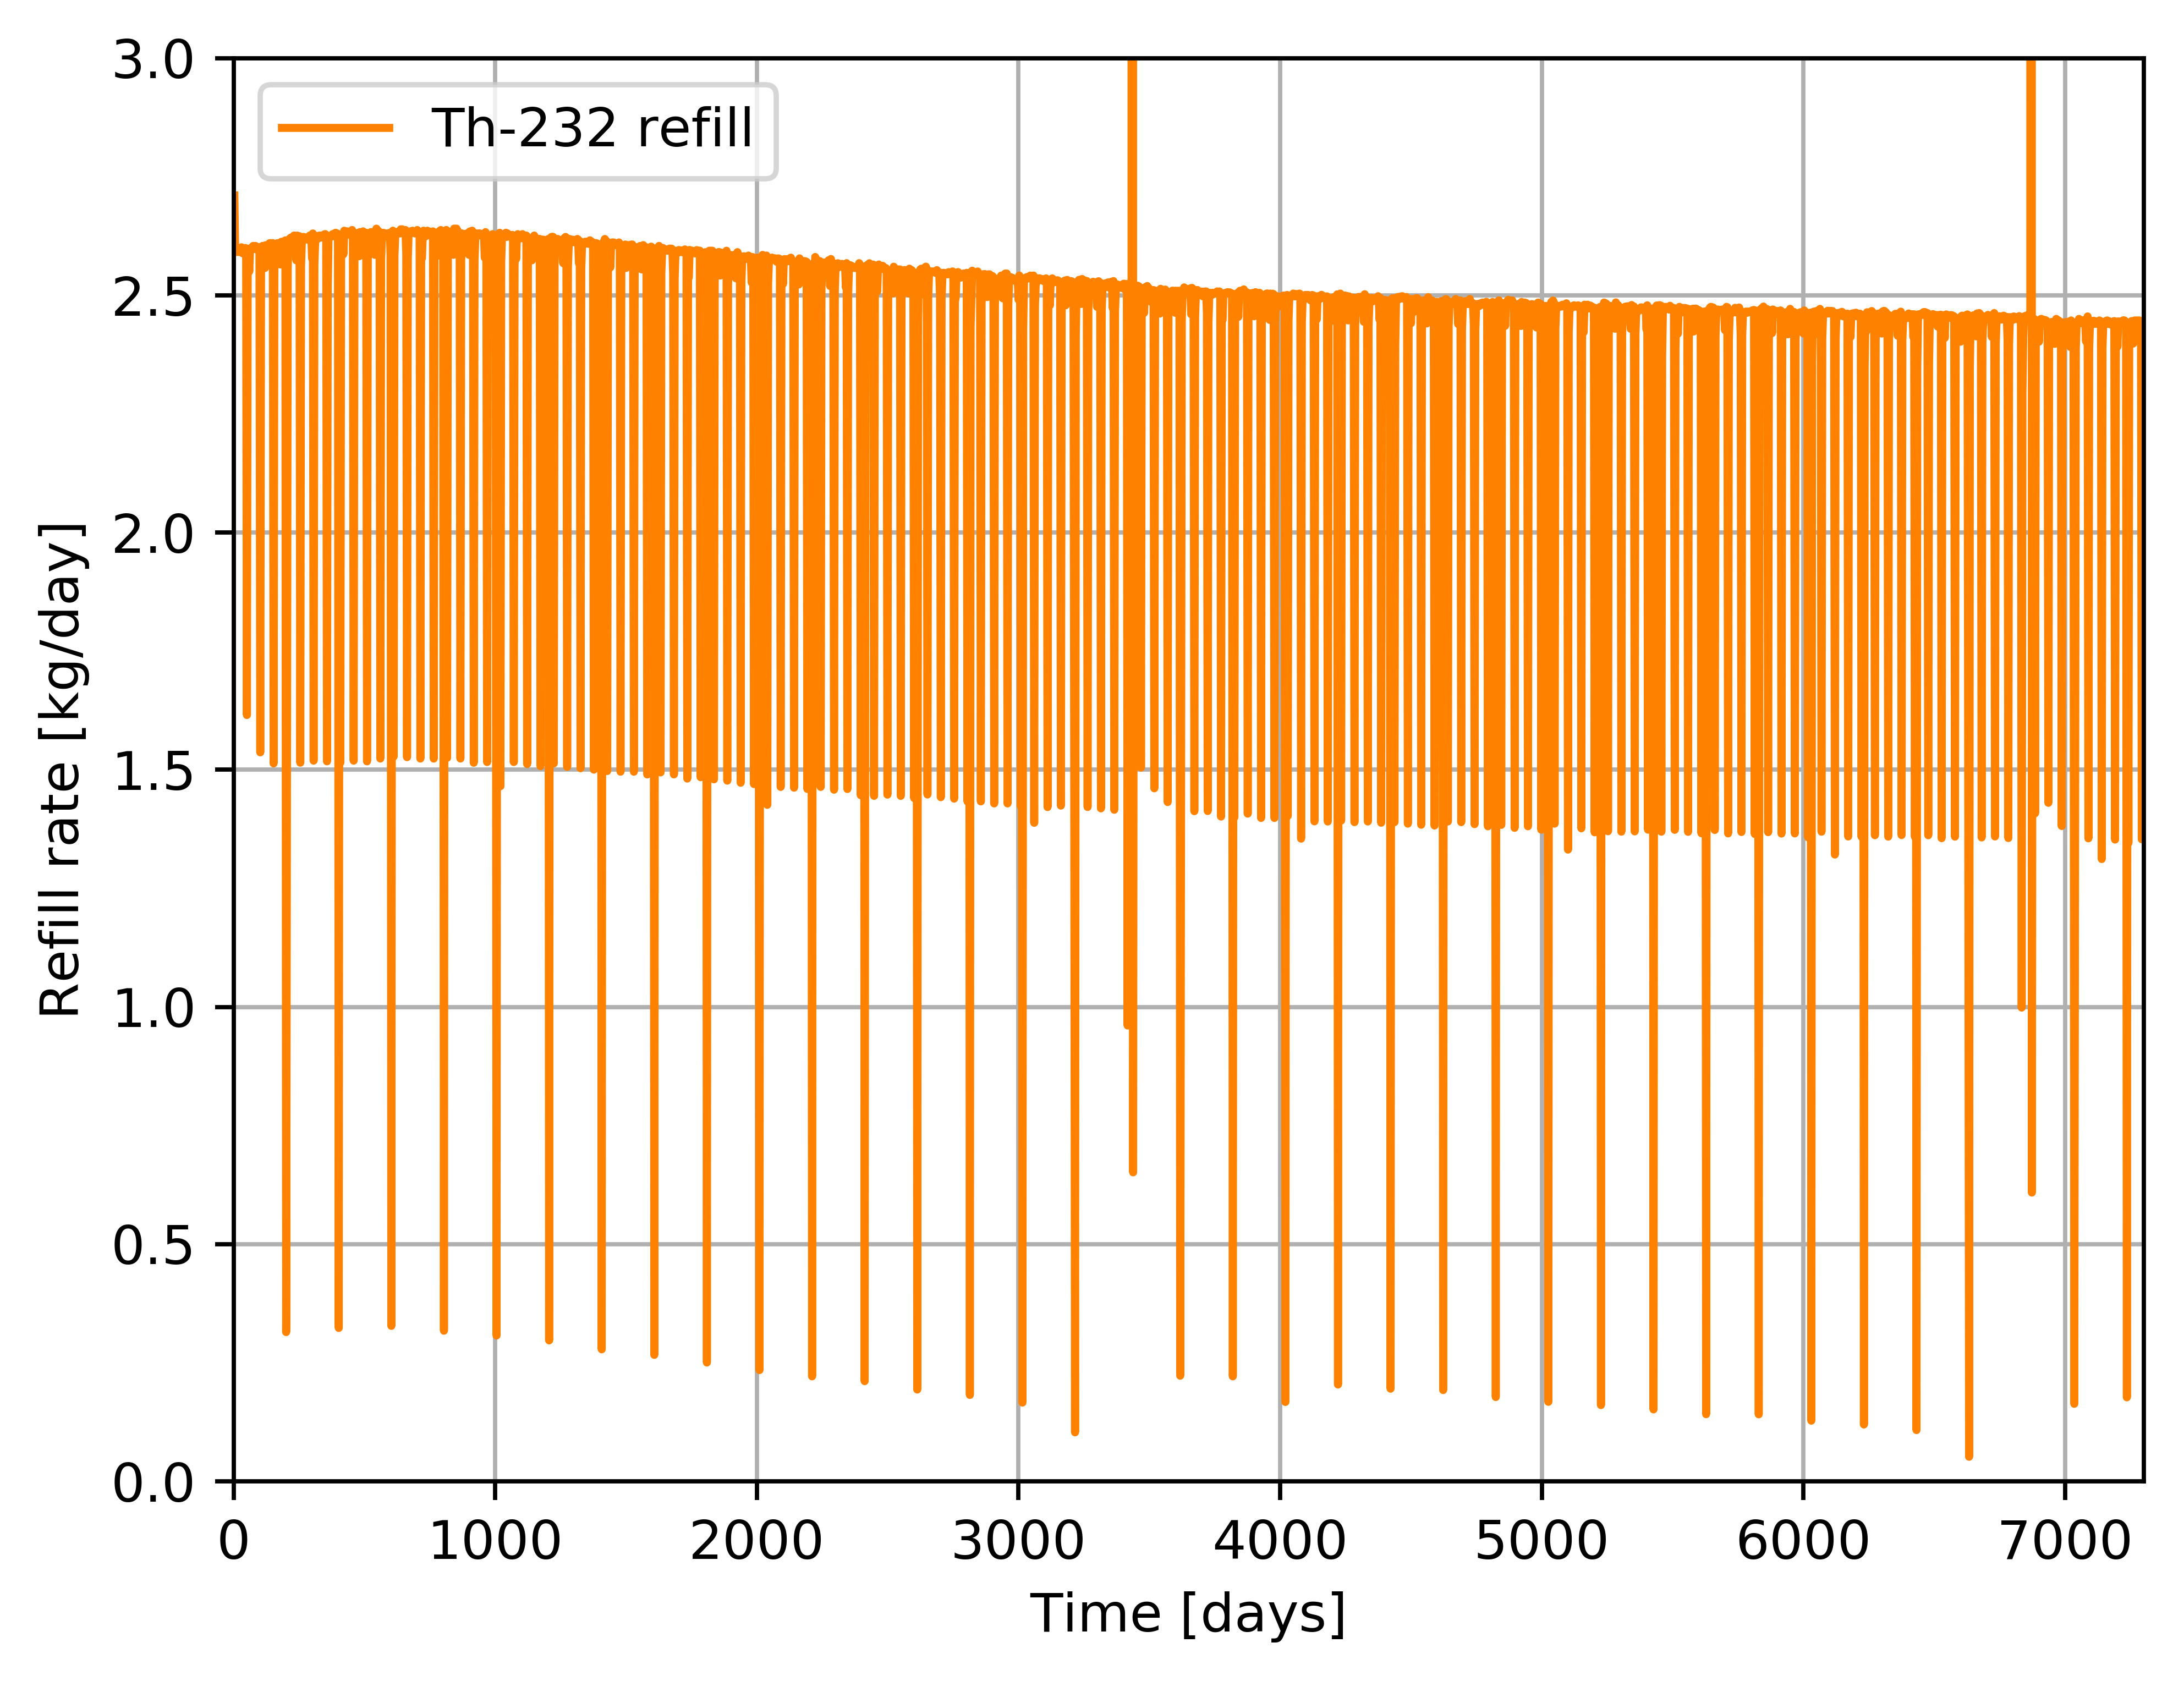
\includegraphics[width=\textwidth]{Th_refill_rate.png} 
      \vspace{-1.5em}
  \caption{$^{232}$Th feed rate over 20 years of \gls{MSBR} operation.}
    \vspace{-0.6em}
  \label{fig:th_refill}
\end{figure}
\begin{figure}[htp!] % replace 't' with 'b' to force it to 
  \centering
    \vspace{-0.3em}
  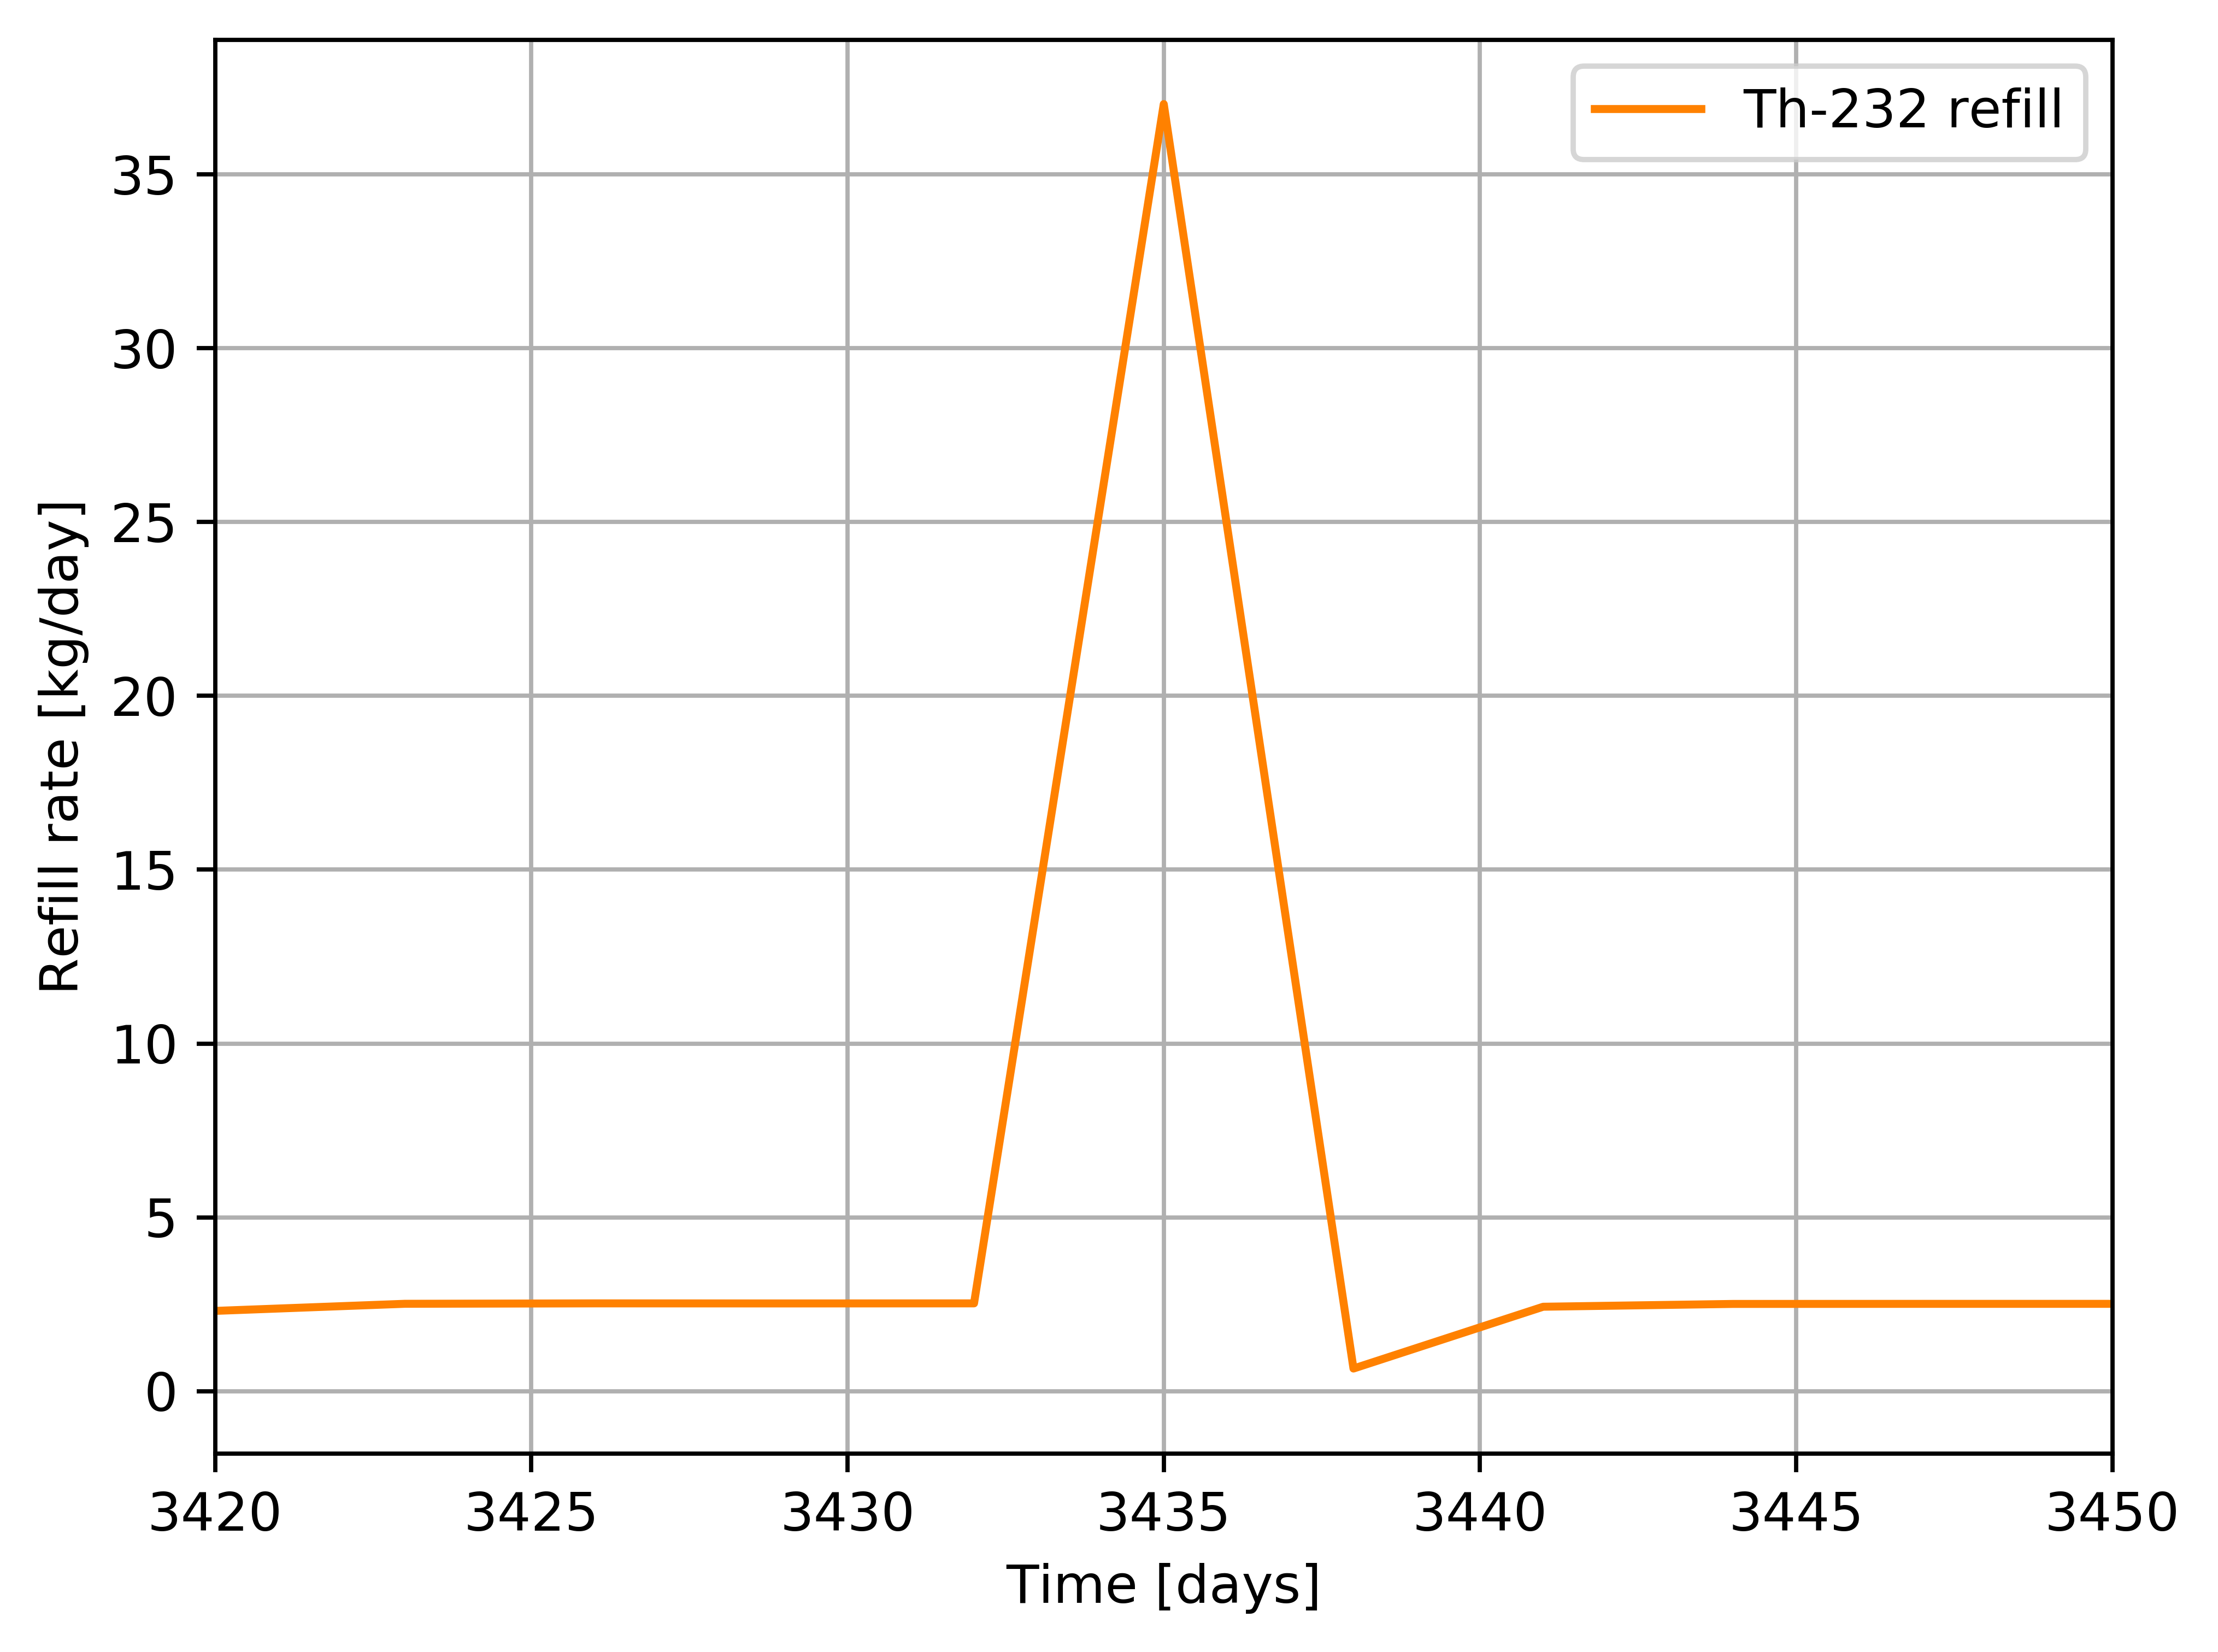
\includegraphics[width=\textwidth]{Th_refill_rate_spike.png} 
      \vspace{-1.5em}
  \caption{Typical $^{232}$Th feed rate spike caused by strong absorbers (Rb, Sr, Cs, Ba) removal.}
    \vspace{-0.6em}
  \label{fig:th_refill_spike}
\end{figure}
\FloatBarrier
